%%
%% Revised ForeSplat manuscript for the COMPAG special issue on foundation models in agriculture.
%% Main revision: the manuscript has been repositioned from an FSAM3/engineering workflow paper
%% to a VFM-guided foreground-prior adaptation and foreground-object 2DGS reconstruction paper.

\documentclass[a4paper]{cas-sc}

\usepackage[numbers,sort&compress,super]{natbib}
\usepackage{tabularx}
\usepackage{amsmath,amssymb}
\usepackage[section]{placeins}
\usepackage{float}
\usepackage{lineno}

% The CAS class enables fleqn by default; switch display equations back to centered.
\makeatletter
\@fleqnfalse
\makeatother

% Keep large figures close to their discussion instead of accumulating at the end.
\setcounter{topnumber}{5}
\setcounter{bottomnumber}{4}
\setcounter{totalnumber}{8}
\renewcommand{\topfraction}{.95}
\renewcommand{\bottomfraction}{.85}
\renewcommand{\textfraction}{.05}
\renewcommand{\floatpagefraction}{.75}
\setlength{\textfloatsep}{10pt plus 2pt minus 2pt}
\setlength{\floatsep}{8pt plus 2pt minus 2pt}
\setlength{\intextsep}{8pt plus 2pt minus 2pt}
\raggedbottom

%%%Author macros
\def\tsc#1{\csdef{#1}{\textsc{\lowercase{#1}}\xspace}}
\tsc{WGM}
\tsc{QE}
%%%

\begin{document}
\let\WriteBookmarks\relax
\linenumbers

\shorttitle{VFM-guided ForeSplat for plant phenotyping}
\shortauthors{Fang et al.}

\title [mode = title]{ForeSplat: Vision-Foundation-Model-Guided Foreground-Object 2D Gaussian Splatting for Low-Cost 3D Plant Phenotyping}

\author[1,2,3,4]{Jian Fang}

\author[2,3,4]{Nengfu Xie}
\cormark[1]

\author[1]{Yane Duan}
\cormark[1]

\author[2,3,4]{Jingchao Fan}
\author[2,3,4]{Xiaoli Wang}
\author[2,3,4]{Hailong Liu}
\author[2,3,4]{Yue Wang}
\author[2,3,4]{Hao Wu}
\author[2,3,4]{Zhibo Meng}
\author[2,3,4]{Xin Wang}
\author[2,3,4]{Rui Man}

\affiliation[1]{organization={College of Intelligent Science and Engineering, Beijing University of Agriculture},
            city={Beijing},
            postcode={102206},
            country={China}}

\affiliation[2]{organization={Agricultural Information Institute, Chinese Academy of Agricultural Sciences},
            city={Beijing},
            postcode={100081},
            country={China}}

\affiliation[3]{organization={National Agricultural Science Data Center},
            city={Beijing},
            postcode={100081},
            country={China}}

\affiliation[4]{organization={Data Hub, Chinese Agrosystem Long-Term Observation Network},
            city={Beijing},
            postcode={100081},
            country={China}}

\cortext[1]{Corresponding authors.}

\begin{abstract}
Vision foundation models (VFMs) provide a new opportunity to reduce annotation and interaction costs in agricultural perception. However, directly applying promptable segmentation models to multiview plant phenotyping is limited by prompt sensitivity, foreground-boundary instability and the mismatch between two-dimensional masks and three-dimensional measurement objects. This paper presents ForeSplat, a VFM-guided foreground-object 2D Gaussian Splatting workflow for low-cost 3D plant phenotyping. We first introduce RAP-FSAM3, a reconstruction-aware prompt-adaptive foreground prior generator that adapts VFMs to potted-plant scenes through semantic-gated multi-prompt selection, structure-balanced foreground--background prompt refinement and geometry-consistency foreground correction. RAP-FSAM3 achieved an F1-score of 0.9706, an mIoU of 0.9641, an HD95 of 183.42 px, a Boundary-F1 of 0.4643 and a leakage energy of 0.001739 on manually annotated evaluation frames sampled from all 20 RGB sequences, outperforming single-prompt SAM3 and other automatic VFM baselines particularly in boundary consistency and leakage suppression. We then convert the VFM-derived foreground priors into 2DGS training-time constraints, including foreground-track initialisation, foreground RGB supervision, opacity constraints, view-quality weighting, a lightweight M2M3-GO primitive-level refinement layer and mask-guided Gaussian pruning. Objective ablation showed that foreground RGB supervision reduced the outside-mask non-black ratio from 0.9908 to 0.0294 and the leakage energy ratio from 1.2201 to 0.0190, whereas post hoc mask pruning after full-scene training remained insufficient. Across 20 RGB multiview sequences and 21 potted plants, ForeSplat achieved PSNR = 31.09 dB, SSIM = 0.9711 and LPIPS = 0.0365, while virtual measurements of plant height, canopy width, leaf length and leaf width agreed with manual measurements with \(R^2\) values of 0.988, 0.988, 0.974 and 0.900. These results indicate that VFMs can support low-cost 3D plant phenotyping when their outputs are adapted as reconstruction-aware foreground priors and injected into the 2DGS optimisation objective.
\end{abstract}

\begin{keywords}
vision foundation model \sep 2D Gaussian Splatting \sep foreground-object reconstruction \sep plant phenotyping \sep RGB imaging
\end{keywords}

\maketitle

\section{Introduction}\label{sec:introduction}

Plant phenotyping provides a technical bridge between genotype, environmental response and agronomic performance. Structural traits such as plant height, canopy width, leaf length and leaf width are widely used in breeding selection, cultivation management and growth assessment \cite{ref6,ref56,ref61}. Manual measurement is labour-intensive, low-throughput and sensitive to operator experience, whereas two-dimensional imaging cannot fully represent overlapping leaves, occluded organs and non-planar canopy geometry. Recent low-cost phenotyping systems likewise emphasise the need for accessible, scalable measurement pipelines \cite{ref62,ref63}. Three-dimensional representations are therefore increasingly used to quantify plant structure, organ position and canopy morphology \cite{ref8,ref10}. Recent reviews further show that 3D imaging and reconstruction are becoming central to trait detection and high-throughput phenotyping workflows \cite{ref9,ref11,ref12}. In practical potted-plant and controlled-environment settings, however, low-cost 3D phenotyping remains difficult because thin leaves, weak texture, repeated patterns, local occlusion, mixed flower--leaf structures and backgrounds with similar colours all reduce the robustness of reconstruction and measurement.

Three-dimensional plant phenotyping has expanded from structure from motion, multiview stereo and depth sensing to neural rendering and explicit Gaussian representations. LiDAR and depth-sensing systems can provide accurate point clouds, but their cost, calibration complexity and deployment requirements limit broad use in horticultural facilities and breeding trials \cite{ref14}. Consumer RGB cameras are flexible and inexpensive, but SfM/MVS remains sensitive to view coverage, image sharpness and leaf texture, even as recent low-cost multiview pipelines show that RGB reconstruction can support crop spatial-geometry analysis beyond single-sample measurement \cite{ref18,ref19}. NeRF improves visual reconstruction through continuous radiance fields and compact neural encodings \cite{ref20,ref21,ref22}. Recent plant studies have used NeRF for field and indoor plant geometry assessment \cite{ref25,ref26}. Comparative plant NeRF studies further indicate that neural rendering can support low-cost crop reconstruction under practical acquisition settings \cite{ref59}. 3D Gaussian Splatting (3DGS) and 2D Gaussian Splatting (2DGS) further provide explicit and editable scene representations \cite{ref27,ref28}. Efficient Gaussian variants also explore compression and compact scene representation \cite{ref51,ref52,ref53}. Mini-splatting shows that constrained Gaussian counts can further reduce representation size \cite{ref54}. Plant3R and PlantGaussian show that Gaussian representations can support plant-structure reconstruction and visualisation \cite{ref30,ref31}. Cotton3DGaussians and object-centric 3DGS further extend this route to boll mapping, plant architecture analysis and strawberry phenotyping \cite{ref32,ref33}. These advances also leave a practical agricultural question unresolved: is the reconstructed 3D object the plant object that needs to be measured?

This question is especially important in potted-plant scenes. Standard NeRF, 3DGS and 2DGS usually optimise the appearance of the full image. The model therefore learns the target potted plant together with tables, surrounding objects and background structures. Full-scene reconstruction is reasonable for novel-view synthesis, but uncontrolled background geometry can contaminate mesh extraction and bounding-range computation when the downstream task is plant height, canopy width and leaf-size measurement. In this study, the VFM prior is therefore defined as a foreground-object prior for the potted-plant instance: the visible supporting container may be retained when it is consistently segmented with the plant, whereas tables and surrounding backgrounds are treated as leakage to be suppressed. Recent target-specific and foundation-model-embedded Gaussian representations further show that two-dimensional semantic cues can shape three-dimensional scene representations, although these methods mainly target general scene understanding rather than trait measurement itself \cite{ref68,ref69}. Together, these studies suggest that plant phenotyping needs a tighter coupling between foreground perception and 3D reconstruction.

Vision foundation models provide a promising route for this coupling, and recent work has explored their adaptation to plant phenotyping \cite{ref55}. However, they are not plug-and-play tools for agricultural 3D phenotyping. A single text prompt may include green background, exclude mature structures, miss mixed flower--leaf regions or produce overly conservative masks. Moreover, even a good two-dimensional mask is not automatically a three-dimensional measurement object. The mask must be adapted into a reconstruction-aware foreground prior and then injected into the optimisation problem that allocates Gaussian capacity during training. Beyond pixel-level foreground supervision, Gaussian primitives still require a primitive-level mechanism to determine whether they are supported by the foreground mask, whether they contribute to uncovered foreground regions and whether they should be preserved, densified or removed. This mechanism is important across representative potted-plant morphologies with broad leaves, compact flowering structures, low canopies and boundary-sensitive foreground regions, where mask coverage and Gaussian capacity allocation may interact differently during densification and pruning.

We therefore propose ForeSplat, a VFM-guided foreground-object 2DGS workflow for multiview potted plants. The workflow contains two coupled components. First, RAP-FSAM3 adapts VFM segmentation to agricultural foreground-prior generation through semantic-gated multi-prompt selection, structure-balanced foreground--background prompt refinement and geometry-consistency foreground correction. Second, ForeSplat converts these foreground priors into 2DGS training-time constraints, including foreground-track initialisation, foreground RGB supervision, alpha and background opacity losses, view-quality weighting, a lightweight M2M3-GO primitive-level refinement layer and mask-guided Gaussian pruning. Thus, masks are not used only as post-processing filters. They help define the 3D optimisation target so that the dominant photometric gradients and Gaussian capacity are directed towards the foreground potted-plant instance rather than uncontrolled tables, surrounding objects or backgrounds.

The contributions of this study are as follows:

\begin{enumerate}
\item We propose RAP-FSAM3, a reconstruction-aware prompt-adaptive foreground prior generator that adapts vision foundation models to potted-plant scenes through semantic-gated multi-prompt selection, structure-balanced foreground--background prompt refinement and geometry-consistency foreground correction.
\item We propose ForeSplat, which converts VFM-derived potted-plant foreground priors into 2DGS training-time constraints and incorporates M2M3-GO as a lightweight primitive-level refinement layer for Gaussian keep, densify and prune decisions after the foreground-object reconstruction target has been established.
\item We validate the method through VFM baseline comparison, prompt robustness analysis, RAP-FSAM3 module ablation, VFM-prior injection-position ablation in 2DGS, and manual-to-virtual phenotypic measurement on multiview potted-plant sequences.
\end{enumerate}

\section{Materials and Methods}\label{sec:materials-and-methods}

\subsection{Study Design and Overall Workflow}\label{sec:study-design-and-overall-workflow}

ForeSplat targets a specific agricultural phenotyping task: generating foreground-object meshes from ordinary multiview RGB images for plant height, canopy width and leaf-size measurement. Here, the foreground object refers to the target potted-plant instance used during reconstruction; it may include the visible supporting container when the VFM consistently groups the plant and container as one instance, while external tables and background structures are excluded. The workflow follows the principle of defining the measured plant object before 3D reconstruction. First, RAP-FSAM3 performs quality filtering and VFM-based foreground-prior adaptation on raw frames, producing reconstruction-aware masks aligned with training views. Second, COLMAP estimates camera poses and sparse point tracks, and multiview mask consistency filters foreground initialisation points. Third, foreground-object 2DGS restricts RGB loss to foreground-instance pixels and constrains the opacity field with alpha mask loss and background opacity loss. Fourth, view-quality-aware soft loss weighting retains all views while modulating their training contributions. Fifth, a lightweight M2M3-GO refinement layer links pixel-level foreground priors with Gaussian-level keep, densify and prune decisions, and mask-guided multi-cue Gaussian pruning together with TSDF mesh extraction produces compact and measurable plant meshes. The overall workflow is shown in Fig.~\ref{fig:workflow}.

\begin{figure}[pos=!htbp]
\centering
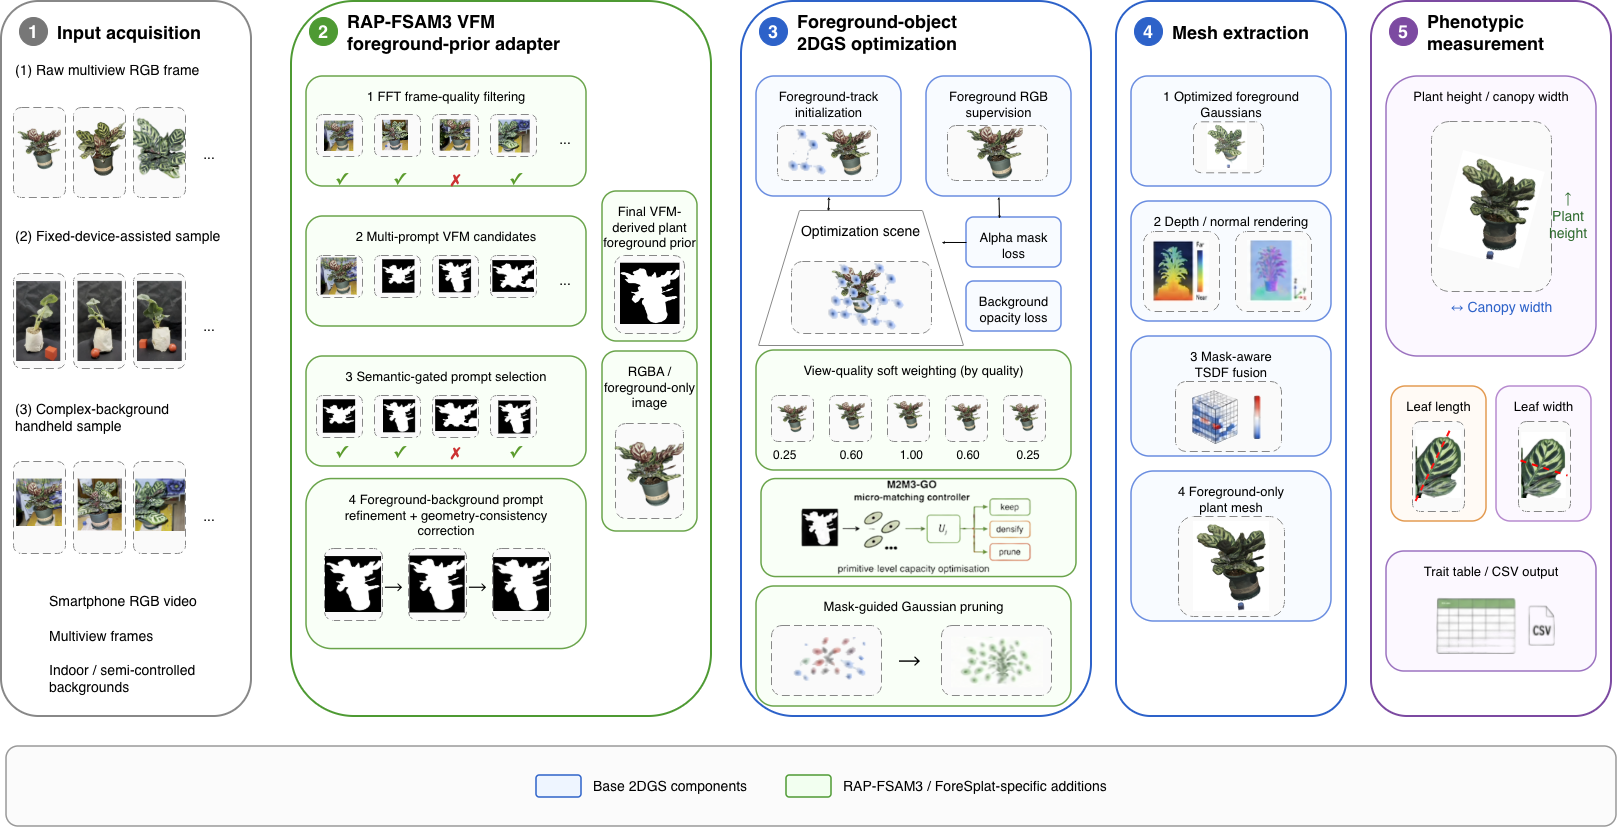
\includegraphics[width=\textwidth,height=0.46\textheight,keepaspectratio]{Fig1.png}
\caption{Overview of the proposed VFM-guided ForeSplat workflow. RAP-FSAM3 adapts VFM outputs into reconstruction-aware potted-plant foreground priors, and ForeSplat injects these priors into 2DGS optimisation to produce foreground-object meshes and virtual trait measurements. M2M3-GO further refines Gaussian keep, densify and prune decisions through bidirectional mask--model micro-matching after the foreground-object target has been established.}\label{fig:workflow}
\end{figure}

\FloatBarrier

\subsection{Dataset, Acquisition Settings and Evaluation Protocol}\label{sec:dataset-acquisition-settings-and-sample}

The full dataset included 20 multiview RGB sequences covering broad leaves, low canopies, overlapping leaves, compact canopies, mixed flowers and leaves, thick leaves, fine texture and dense occlusion. Images were acquired with an iPhone 14 Pro Max at a video resolution of 1080 x 1920 and a frame rate of 60 fps. Two acquisition settings were used: fixed-device-assisted capture and handheld circular capture in complex indoor backgrounds. All 20 sequences were used for full-workflow validation. Phenotypic statistics were analysed at the plant level for 21 plants; leaf length and leaf width were measured on three representative leaves per plant, giving \(n = 63\) for leaf traits. For foreground-prior evaluation, we sampled and manually annotated evaluation frames from all 20 RGB sequences. These annotated frames covered all plant samples and both acquisition settings, and were used consistently for VFM comparison, prompt robustness analysis and RAP-FSAM3 module ablation. Dataset use and evaluation blocks are summarised in Table~\ref{tab:dataset-protocol}, and acquisition coverage and workflow execution are reported in Table~\ref{tab:dataset-coverage}.

\begin{table}[pos=!htbp]
\caption{Dataset use and evaluation protocol. The foreground-prior rows refer to manually annotated evaluation frames sampled from all 20 RGB sequences.}\label{tab:dataset-protocol}
\centering
\scriptsize
\setlength{\tabcolsep}{4pt}
\resizebox{\textwidth}{!}{%
\begin{tabular}{@{}lccc@{}}
\toprule
Evaluation block & Samples & Frames / plants & Purpose \\
\midrule
VFM foreground-prior evaluation & All 20 RGB multiview sequences & Manually annotated evaluation frames & VFM baseline comparison and prompt robustness \\
RAP-FSAM3 module ablation & All 20 RGB multiview sequences & Manually annotated evaluation frames & Contribution analysis of foreground-prior adaptation modules \\
Full reconstruction validation & 20 RGB multiview sequences & 20 reconstruction samples & Workflow-level 3D reconstruction and mesh generation \\
Phenotypic validation & 21 plants & 21 plant-level traits and 63 leaf-level traits & Manual-to-virtual trait agreement \\
\bottomrule
\end{tabular}%
}
\end{table}

\begin{table}[pos=!htbp]
\caption{Dataset coverage and end-to-end workflow execution for the two acquisition settings.}\label{tab:dataset-coverage}
\centering
\scriptsize
\setlength{\tabcolsep}{3pt}
\resizebox{\textwidth}{!}{%
\begin{tabular}{@{}lccccccc@{}}
\toprule
Setting & Species/cultivar labels & Samples & Raw frames & Effective frames & SfM-registered views & Successful samples & Success rate \\
\midrule
Fixed-device-assisted capture & 8 & 10 & 2502 & 2104 & 2040 & 10 & 100\% \\
Complex-background capture & 7 & 10 & 2500 & 2113 & 2089 & 10 & 100\% \\
\bottomrule
\end{tabular}%
}
\end{table}

\FloatBarrier

\subsection{RAP-FSAM3: Reconstruction-Aware Prompt-Adaptive Foreground Priors}\label{sec:rap-fsam3}

RAP-FSAM3 is designed to generate potted-plant foreground priors for 3D reconstruction rather than to serve as an independent general segmentation model. Its input is the raw multiview RGB frames of each plant. Its outputs are binary masks, alpha images and foreground-instance RGB images aligned one-to-one with the training images. RAP-FSAM3 first removes severely blurred frames through frequency-domain quality filtering and then adapts VFM masks to the reconstruction task through multi-prompt candidate generation, semantic-gated selection, foreground--background prompt refinement and geometry-consistency correction.

\subsubsection{FFT-Based Frame-Quality Filtering}\label{sec:fft-based-frame-quality-filtering}

Blurred, defocused and weakly textured frames can affect SfM pose estimation, VFM mask boundaries and subsequent 2DGS optimisation. We computed the two-dimensional FFT magnitude spectrum for each frame and used a normalised high-frequency saliency index rather than an absolute high-frequency sum:

\[
Q_{\text{FFT}}(I)=
\frac{\left\| W_H\odot \log\left(1+\left|\mathcal{F}(I)\right|\right)\right\|_1}
{\left\| \log\left(1+\left|\mathcal{F}(I)\right|\right)\right\|_1+\varepsilon} .
\]

Here, \(I\) denotes the input frame after conversion to grayscale for quality evaluation, and \(\mathcal{F}(I)\) denotes its two-dimensional Fourier transform. The term \(|\mathcal{F}(I)|\) is the magnitude spectrum, and \(\log(1+|\mathcal{F}(I)|)\) compresses the dynamic range of the spectrum so that a few extremely strong low-frequency components do not dominate the score. \(W_H\in[0,1]^{H\times W}\) is a radial high-pass weighting mask, where entries close to the spectral centre receive low weights and high-frequency regions receive large weights. The operator \(\odot\) denotes element-wise multiplication, \(\|\cdot\|_1\) sums the weighted spectral responses, and \(\varepsilon\) is a small constant used to avoid division by zero. Therefore, \(Q_{\text{FFT}}(I)\) is a normalised high-frequency saliency score: a larger value indicates that the frame contains richer edges and details and is less likely to be severely blurred. The distribution of \(Q_{\text{FFT}}\) was computed independently for each sequence, and the first quartile was used as a sample-adaptive threshold. Frames below this threshold were excluded from subsequent segmentation and COLMAP processing.

\subsubsection{Multi-Prompt VFM Candidate Generation}\label{sec:multi-prompt-vfm-candidates}

Frames that passed quality filtering were input to the VFM. Promptable segmentation models have shown strong general foreground localisation in natural-image and video segmentation \cite{ref38,ref39,ref71}. Plant point-cloud segmentation studies indicate that learned 3D segmentation can support organ-level structural analysis \cite{ref42,ref43}. Recent open-vocabulary methods have broadened prompt-based object perception for complex scenes \cite{ref40,ref64}. Point Transformer V3 further strengthens general-purpose 3D representation learning \cite{ref44}. For each frame \(I_i\), RAP-FSAM3 queries the VFM using five plant-related prompts: a green-region prompt, \texttt{green\ plant}; a plant-instance prompt, \texttt{entire\ potted\ plant}; an organ-level prompt, \texttt{leaves\ and\ stems}; a seedling-oriented prompt, \texttt{crop\ seedling}; and a background-excluding plant prompt, \texttt{plant\ body\ without\ background}. These prompts produce a candidate mask set

\[
\mathcal{M}_i=\left\{M_i^{(1)},M_i^{(2)},\ldots,M_i^{(K)}\right\}, \quad K=5.
\]

Here, \(i\) is the frame index, \(k\) is the prompt index, \(K=5\) is the number of plant-related prompts, and \(M_i^{(k)}\in\{0,1\}^{H\times W}\) is the binary foreground mask predicted for frame \(I_i\) using the \(k\)-th prompt. The five candidates correspond to the green-region, plant-instance, organ-level, seedling-oriented and background-excluding plant prompts, respectively. The plant-instance prompt is defined as a potted-plant foreground prompt rather than a strict plant-body-only prompt, because in the collected scenes the VFM often treats the plant and its visible supporting container as one coherent foreground instance. This design allows the method to expose and handle prompt-induced semantic bias instead of relying on a single fixed textual description.

\subsubsection{Semantic-Gated Multi-Prompt Selection}\label{sec:semantic-gated-selection}

A naive prompt selector that considers only mask geometry may choose a semantically inappropriate candidate, such as an organ-only or seedling-oriented mask in a mature potted plant. RAP-FSAM3 therefore uses semantic-gated multi-prompt selection. For each candidate mask, we construct a foreground-prior descriptor

\[
\boldsymbol{\phi}_i^{(k)}=\left[
q_{\text{plant}},\ q_{\text{area}},\ q_{\text{comp}},\ q_{\text{edge}},\ q_{\text{contrast}},\ q_{\text{temp}}
\right]^{\top},
\]

and an interference descriptor

\[
\boldsymbol{\psi}_i^{(k)}=\left[
q_{\text{table}},\ q_{\text{bg}},\ q_{\text{neighbour}},\ q_{\text{outlier}}
\right]^{\top}.
\]

The semantic compatibility of the \(k\)-th candidate is modelled as a gated confidence score

\[
c_i^{(k)}=\sigma\!\left(
\mathbf{w}_{\phi}^{\top}\boldsymbol{\phi}_i^{(k)}
-\mathbf{w}_{\psi}^{\top}\boldsymbol{\psi}_i^{(k)}-b
\right),
\]

In these equations, \(\boldsymbol{\phi}_i^{(k)}\) describes the foreground reliability of the \(k\)-th candidate in frame \(i\). Specifically, \(q_{\text{plant}}\) measures plant-body semantic evidence, \(q_{\text{area}}\) measures whether the foreground area lies in a reasonable range, \(q_{\text{comp}}\) penalises fragmented connected components, \(q_{\text{edge}}\) measures boundary clarity, \(q_{\text{contrast}}\) measures foreground-background appearance separability, and \(q_{\text{temp}}\) measures temporal consistency with neighbouring frames. The vector \(\boldsymbol{\psi}_i^{(k)}\) describes external interference evidence, where \(q_{\text{table}}\), \(q_{\text{bg}}\), \(q_{\text{neighbour}}\) and \(q_{\text{outlier}}\) measure the degree to which the candidate leaks into table regions, distant background regions, neighbouring plants and isolated outlier fragments. The visible pot is not treated as a negative class in this prompt-robustness setting when it is consistently returned as part of the target potted-plant instance. \(\mathbf{w}_{\phi}\) and \(\mathbf{w}_{\psi}\) are weighting vectors for foreground reliability and interference evidence, \(b\) is a bias term, and \(\sigma(\cdot)\) is the sigmoid function that maps the semantic compatibility score to \([0,1]\). Thus, \(c_i^{(k)}\) represents the semantic compatibility of the \(k\)-th candidate. Candidate reliability is then normalised through a temperature-controlled softmax,

\[
a_i^{(k)}=\frac{\exp\left(c_i^{(k)}/\tau_s\right)}
{\sum_{l=1}^{K}\exp\left(c_i^{(l)}/\tau_s\right)} ,
\]

where \(a_i^{(k)}\) is the normalised reliability assigned to the \(k\)-th candidate and \(\tau_s\) is the softmax temperature controlling how sharply the method selects among prompts. A smaller \(\tau_s\) makes the selection closer to a hard argmax, whereas a larger value makes the reliability distribution smoother. The final selected prior is

\[
M_i^{*}=M_i^{(k^{*})},\qquad
k^{*}=\arg\max_{k} a_i^{(k)} .
\]

Here, \(k^*\) is the selected prompt index and \(M_i^*\) is the selected VFM foreground prior for frame \(i\). This semantic gate acts as a safety mechanism: it does not necessarily increase the average region-overlap score by itself, but it prevents semantically inconsistent prompt choices before further refinement. The softmax form also makes the confidence distribution over prompts explicit, which is useful for prompt-robustness analysis.

\subsubsection{Structure-Balanced Foreground--Background Prompt Refinement}\label{sec:foreground-background-refinement}

The selected candidate mask is further refined through structure-balanced foreground--background prompt refinement. Positive prompts are sampled from the main foreground instance, including the plant body and the consistently visible support base when present, while negative prompts are sampled from external table, background, neighbouring-plant and expansion-ring regions around the candidate mask. Let \(d_{M_i^{*}}(p)\) denote the distance-transform value from pixel \(p\) to the boundary of \(M_i^{*}\). Stable positive prompts are selected from the high-confidence mask interior:

\[
\mathcal{P}_i^{+}=\operatorname{TopK}_{p\in M_i^{*}}
\left(d_{M_i^{*}}(p),K_{+}\right).
\]

where \(\mathcal{P}_i^+\) is the positive prompt set, \(d_{M_i^*}(p)\) is the distance-transform value from pixel \(p\) to the boundary of the selected mask, \(K_+\) is the number of positive prompts, and \(\operatorname{TopK}\) selects the pixels with the largest distance values. Pixels with larger \(d_{M_i^*}(p)\) are farther from uncertain boundaries and therefore provide more reliable positive prompts from the plant interior. The negative prompt candidate region is defined as

\[
\mathcal{R}_i^{-}=\left(\operatorname{Dilate}\left(M_i^{*},r\right)\setminus M_i^{*}\right)
\cup \mathcal{I}_{\text{table}}
\cup \mathcal{I}_{\text{bg}}
\cup \mathcal{I}_{\text{neighbour}},
\]

Here, \(\mathcal{R}_i^-\) is the candidate region for negative prompts. \(\operatorname{Dilate}(M_i^*,r)\setminus M_i^*\) is an expansion ring around the selected foreground-instance boundary, where \(r\) is the dilation radius; this ring captures pixels that are spatially close to the foreground boundary and are likely to contain table, neighbouring-object or background leakage. \(\mathcal{I}_{\text{table}}\), \(\mathcal{I}_{\text{bg}}\) and \(\mathcal{I}_{\text{neighbour}}\) denote potential table, distant-background and neighbouring-plant interference regions. The visible container is not used as a negative prompt when it is consistently included in the selected potted-plant instance. Negative prompts are sampled by non-maximum suppression over the interference score \(\zeta_i(p)\):

\[
\mathcal{P}_i^{-}=\operatorname{NMS}_{p\in\mathcal{R}_i^{-}}
\left(\zeta_i(p),K_{-},r_{\text{nms}}\right).
\]

In this operation, \(\mathcal{P}_i^-\) is the selected set of negative prompts, \(K_-\) is the maximum number of negative prompts, and \(r_{\text{nms}}\) is the non-maximum suppression radius used to avoid clustered negative points. \(\zeta_i(p)\) gives a higher score to pixels that are more likely to be background or interfering structures. The complete prompt set is therefore

\[
\mathcal{P}_i=\left(\mathcal{P}_i^{+},\mathcal{P}_i^{-}\right).
\]

Here, \(\mathcal{P}_i^+\) and \(\mathcal{P}_i^-\) are positive and negative prompt sets, respectively, and \(\mathcal{P}_i\) is the structured prompt set used for VFM refinement. The VFM is then re-queried or refined using \(\mathcal{P}_i\), producing a foreground prior that better separates the target potted-plant instance from surrounding tables, neighbouring plants and background regions. Compared with a simple union of positive and negative prompts, this formulation explicitly encodes spatial confidence, interference regions and prompt diversity.

\subsubsection{Geometry-Consistency Foreground Correction}\label{sec:geometry-consistency-correction}

Finally, RAP-FSAM3 applies geometry-consistency foreground correction. Sparse geometric support from COLMAP and the 2DGS pipeline is used to recover mask-external pixels that are supported by multiview geometry. Let \(X_j\) be a sparse point visible in view \(i\), and let \(\pi_i(X_j)\) denote its projection. We first build a differentiable projection-support field

\[
H_i(p)=\sum_{X_j\in X_i}\omega_{ij}\,
\kappa_{\sigma}\!\left(p-\pi_i(X_j)\right),
\]

Here, \(H_i(p)\) is the geometric support field at pixel \(p\) in view \(i\), \(X_i\) is the set of sparse 3D points visible in that view, \(X_j\) is one visible sparse point, and \(\pi_i(X_j)\) is its 2D projection. \(\kappa_{\sigma}(\cdot)\) is a Gaussian kernel with bandwidth \(\sigma\), which spreads each sparse projection into a local support region instead of a single pixel. \(\omega_{ij}\) is the geometric reliability weight for the projection, used to down-weight uncertain points or views. The consistency between the current mask and the sparse geometric support is measured by the normalised overlap

\[
G_i=\frac{\left\langle H_i,M_i\right\rangle}
{\left\|H_i\right\|_1+\varepsilon}.
\]

In this equation, \(G_i\) measures how much of the sparse geometric support is covered by the current mask. \(\langle H_i,M_i\rangle\) denotes the inner product between the support field and the mask, and \(\|H_i\|_1\) normalises the score by the total geometric support. A conservative positive correction is applied only in a boundary neighbourhood \(\mathcal{B}_i=\operatorname{Dilate}(M_i,r_g)\setminus\operatorname{Erode}(M_i,r_g)\):

\[
M_i^{\text{geo}}=M_i\ \vee\ 
\left[\mathbf{1}\left(H_i>\tau_g\right)\odot\mathbf{1}\left(p\in\mathcal{B}_i\right)\right].
\]

Here, \(M_i^{\text{geo}}\) is the geometry-corrected foreground prior, \(\vee\) denotes logical OR, \(\mathbf{1}[\cdot]\) is an indicator function, \(\tau_g\) is the geometric support threshold, and \(p\in\mathcal{B}_i\) restricts the correction to the uncertain boundary band. Negative deletion is disabled by default to avoid damaging thin leaves, petioles and narrow boundary structures. This correction is intended mainly to improve extreme-boundary consistency rather than to act as the main source of segmentation gain. The complete RAP-FSAM3 foreground-prior generation process is summarised in Fig.~\ref{fig:rap-fsam3}.

\begin{figure}[pos=!htbp]
\centering
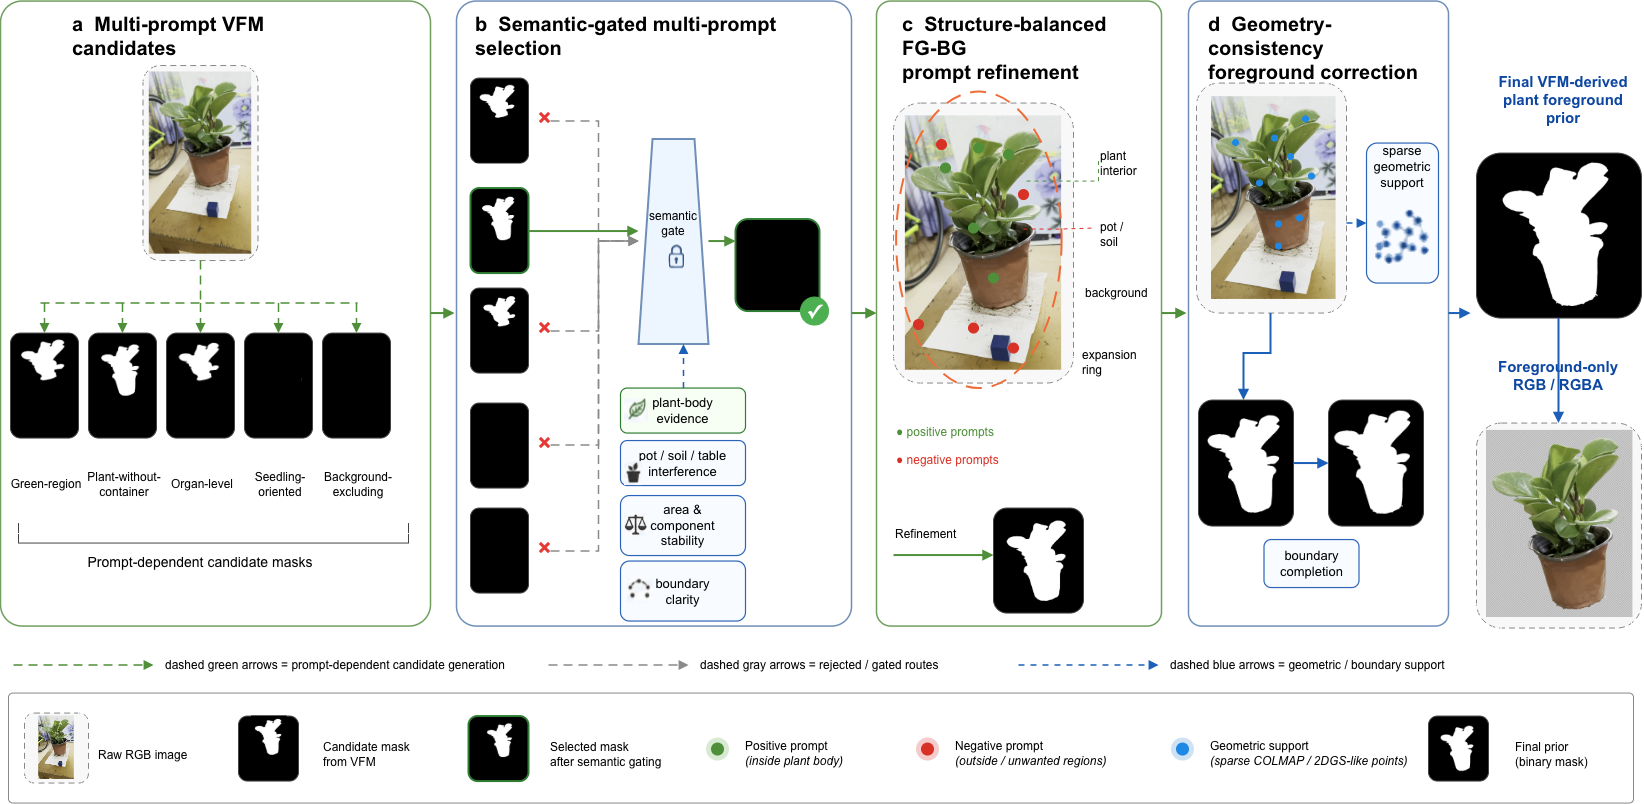
\includegraphics[width=\textwidth,height=0.46\textheight,keepaspectratio]{Fig2.png}
\caption{RAP-FSAM3 foreground-prior generation. The module adapts VFM outputs to potted-plant reconstruction through semantic-gated multi-prompt selection, structure-balanced foreground--background prompt refinement and geometry-consistency foreground correction.}\label{fig:rap-fsam3}
\end{figure}
\FloatBarrier

\subsection{Foreground-Object 2DGS Optimisation}\label{sec:foreground-object-2dgs}

RAP-FSAM3 produces reconstruction-aware VFM foreground priors. ForeSplat then converts these priors into training-time constraints for 2DGS. With this prior, the reconstruction target is shifted from full-scene appearance to the potted-plant foreground object. Foreground trajectory initialisation and foreground RGB supervision constrain the optimisation object. Alpha and background opacity constraints, together with view-quality soft weighting, stabilise training. M2M3-GO further refines Gaussian-level keep, densify and prune decisions, and mask-guided pruning cleans redundant primitives before exporting a foreground-object TSDF mesh.



\subsubsection{Camera Pose Estimation and Foreground Trajectory Initialisation}\label{sec:camera-pose-estimation-and-foreground-tr}

Camera intrinsics, extrinsics and sparse 3D point tracks were estimated using the incremental SfM pipeline in COLMAP \cite{ref16}. Standard 2DGS initialises Gaussian primitives from all sparse points, so background points enter the representation before optimisation begins. ForeSplat filters sparse points through confidence-weighted multiview mask consistency. Let sparse point \(X_j\) be visible in a view set \(V_j\), and let its projection in view \(i\) be \(\pi_i(X_j)\). We define the foreground-track confidence as

\[
\Gamma(X_j)=
\frac{\sum_{i\in V_j}\omega_{ij}^{\text{trk}}\,
M_i\!\left(\pi_i(X_j)\right)}
{\sum_{i\in V_j}\omega_{ij}^{\text{trk}}+\varepsilon},
\]

Here, \(\Gamma(X_j)\) is the foreground-track confidence of sparse point \(X_j\), \(V_j\) is the set of views in which \(X_j\) is visible, and \(M_i(\pi_i(X_j))\) indicates whether the projection of \(X_j\) lies inside the foreground prior in view \(i\). The weight \(\omega_{ij}^{\text{trk}}\) can encode reprojection reliability, visibility and view-quality confidence, and \(\varepsilon\) avoids division by zero. The retention criterion is

\[
\operatorname{Keep}(X_j)=\mathbf{1}\left[
|V_j|\geq 3\ \land\ \Gamma(X_j)\geq \tau_{\text{track}}
\right].
\]

In this criterion, \(\operatorname{Keep}(X_j)\) is a binary decision indicating whether the sparse point is retained for Gaussian initialisation, \(|V_j|\geq 3\) enforces multiview support, \(\Gamma(X_j)\geq\tau_{\text{track}}\) enforces foreground consistency, and \(\tau_{\text{track}}\) is the track-consistency threshold. Foreground trajectory initialisation required each sparse point to be observed in at least 3 views. We set \(\tau_{\text{track}}=0.9\) and used no mask dilation.

\subsubsection{Foreground RGB Supervision and Opacity Constraints}\label{sec:foreground-rgb-supervision-and-opacity-c}

Standard 2DGS optimises RGB reconstruction over the full image domain \(\Omega\) \cite{ref28}. For potted-plant phenotyping, this allows tables, surrounding objects and background structures to compete with the target foreground instance for model capacity. ForeSplat therefore redefines photometric supervision on the potted-plant foreground prior. The standard full-image RGB loss can be written as an empirical risk over all pixels:

\[
L_{\text{rgb-full}}=
\mathbb{E}_{p\sim\Omega}\left[\rho_{\text{rgb}}\left(R(p)-I(p)\right)\right],
\]

Here, \(p\sim\Omega\) means that pixels are sampled from the full image domain \(\Omega\), \(R(p)\) is the rendered colour at pixel \(p\), \(I(p)\) is the observed input colour, and \(\rho_{\text{rgb}}(\cdot)\) is implemented as an \(L_1\) photometric penalty. This full-image objective treats the target potted-plant instance and uncontrolled background regions as equally valid reconstruction targets. ForeSplat replaces this full-scene risk with a foreground-conditioned risk. Let

\[
w_M(p)=M(p)\,\mathbf{1}\left[\operatorname{dist}\left(p,\partial M\right)>r_b\right]
\]

be a valid foreground supervision weight that ignores a narrow uncertain boundary band. In this definition, \(M(p)\) is the VFM-derived foreground prior at pixel \(p\), \(\partial M\) is the mask boundary, \(\operatorname{dist}(p,\partial M)\) is the pixel-to-boundary distance, \(r_b\) is the boundary-ignore radius, and the indicator function removes pixels close to uncertain mask boundaries from RGB supervision. Let \(Z_M=\sum_{p\in\Omega}w_M(p)+\varepsilon\) be the normalisation term. The foreground RGB loss is

\[
L_{\text{rgb-fg}}=
\frac{1}{Z_M}\sum_{p\in\Omega}w_M(p)\,
\rho_{\text{rgb}}\left(R(p)-I(p)\right).
\]

In this equation, \(L_{\text{rgb-fg}}\) averages the photometric penalty only over reliable plant-foreground pixels. We further add an alpha mask loss implemented as an \(L_1\)-Dice compound term:

\[
L_{\text{mask}}=
\lambda_{\ell_1}\frac{1}{|\Omega|}\sum_{p\in\Omega}|A(p)-M(p)|
+\lambda_{\text{dice}}\left(1-
\frac{2\langle A,M\rangle+\varepsilon}
{\|A\|_1+\|M\|_1+\varepsilon}
\right),
\]

Here, \(A(p)\) is the rendered alpha value at pixel \(p\), \(\lambda_{\ell_1}\) and \(\lambda_{\text{dice}}\) balance the pixel-wise \(L_1\) term and the Dice-overlap term, \(\langle A,M\rangle\) is the inner product between the rendered alpha map and the foreground prior, and \(\|A\|_1\) and \(\|M\|_1\) denote their summed responses. The Dice term penalises region-level disagreement between the opacity field and the VFM foreground prior. We also add a background opacity suppression term:

\[
L_{\text{bg}}=
\frac{\left\langle 1-M,A\right\rangle}
{\|1-M\|_1+\varepsilon} .
\]

where \(1-M\) indicates the background region and \(L_{\text{bg}}\) penalises residual opacity outside the plant foreground. The complete optimisation objective uses a warm-up schedule \(\chi(t)\) for the mask-related terms:

\[
L_{\text{core}}(t)=
L_{\text{rgb-fg}}+
\chi(t)\left(\lambda_{\text{mask}}L_{\text{mask}}
+\lambda_{\text{bg}}L_{\text{bg}}\right)+L_{\text{reg}},
\]

where

\[
\chi(t)=\operatorname{clip}\left(\frac{t-t_0}{T_{\text{warm}}},0,1\right).
\]

Here, \(t\) is the training iteration, \(t_0\) is the iteration at which mask-related constraints begin, \(T_{\text{warm}}\) is the warm-up length, and \(\operatorname{clip}(\cdot,0,1)\) restricts \(\chi(t)\) to \([0,1]\). \(L_{\text{reg}}\) includes the 2DGS depth-distortion loss and normal-consistency loss. \(\lambda_{\text{mask}}\) and \(\lambda_{\text{bg}}\) control the strengths of mask consistency and background opacity suppression. We used \(\lambda_{\text{mask}}=0.08\) and \(\lambda_{\text{bg}}=0.02\). The mask loss type was \texttt{l1\_dice}, mask boundaries of 2 px were ignored, and the mask loss was activated after 500 iterations with a 1500-iteration warm-up.

\subsection{View-Quality-Aware Soft Loss Weighting}\label{sec:view-quality-aware-soft-loss-weighting}

In multiview plant sequences, some views may contain mild blur, specular reflection or local occlusion. Nevertheless, they may still cover thin leaf structures visible only from narrow angles. Directly removing low-quality frames can therefore damage angular coverage. ForeSplat therefore converts a view-quality score \(s_i\), computed from mask coverage, boundary sharpness and foreground RGB contrast, into a bounded reliability weight:

\[
q_i=q_{\min}+(q_{\max}-q_{\min})
\sigma\left(\frac{s_i-\mu_s}{\sigma_s+\varepsilon}\right),
\qquad q_i\in[0.6,1.0].
\]

In this equation, \(q_i\) is the reliability weight of view \(i\), \(s_i\) is the raw view-quality score, \(\mu_s\) and \(\sigma_s\) are the mean and standard deviation of the quality scores within the sequence, and \(q_{\min}\) and \(q_{\max}\) are the lower and upper bounds of the weight range. We set \(q_{\min}=0.6\) and \(q_{\max}=1.0\), so lower-quality views are down-weighted but not removed. The soft-weighted foreground loss is then

\[
L_{\text{rgb-fg-soft}}=\sum_i \bar{q}_i L_{\text{rgb-fg}}(i),\qquad
\bar{q}_i=\frac{q_i}{\sum_l q_l+\varepsilon}.
\]

Here, \(L_{\text{rgb-fg}}(i)\) is the foreground RGB loss of view \(i\), \(\bar{q}_i\) is the normalised reliability weight, and the denominator ensures that weights sum to one across views. ForeSplat uses precomputed view-quality weights and applies \texttt{view\_weight\_mode=rgb\_only}.

\subsection{Mask-Guided Multi-Cue Gaussian Pruning}\label{sec:mask-guided-multi-cue-gaussian-pruning}

Weakly supported Gaussian primitives may remain near object boundaries in late training. For each Gaussian \(g_j\), ForeSplat builds a pruning descriptor

\[
\mathbf{z}_j=\left[
M_j,\ \log(O_j+\varepsilon),\ \log(1+V_j),\ B_j,\ C_j
\right]^{\top},
\]

Here, \(\mathbf{z}_j\) is the pruning descriptor of Gaussian primitive \(g_j\). \(M_j\) denotes mask-projection consistency, \(O_j\) is opacity, \(V_j\) is the number of visible views, \(B_j\) measures colour/brightness normality and \(C_j\) represents local topological cues. The logarithmic transforms reduce the dynamic range of opacity and view-count terms. The primitive survival score is modelled as

\[
P_{\text{keep}}(g_j)=\sigma\left(\mathbf{w}_{g}^{\top}\mathbf{z}_j-b_g\right).
\]

where \(P_{\text{keep}}(g_j)\) is the survival score of the primitive, \(\mathbf{w}_g\) is the cue-weight vector, \(b_g\) is a bias term and \(\sigma(\cdot)\) maps the score to \([0,1]\). A primitive is removed only when its survival score is below a threshold and the per-round removal budget is not exceeded:

\[
\operatorname{Prune}(g_j)=\mathbf{1}\left[
P_{\text{keep}}(g_j)<\tau_g\right]\cdot
\mathbf{1}\left[\frac{N_{\text{removed}}}{N_{\text{all}}}<r_{\max}\right].
\]

In this decision, \(\tau_g\) is the pruning threshold, \(N_{\text{removed}}\) is the number of primitives already removed in the current pruning round, \(N_{\text{all}}\) is the number of primitives before the round, and \(r_{\max}\) is the maximum removal ratio. The pruning module uses \texttt{pruning\_mode=mask}, starts at 18,000 iterations and is executed every 3,000 iterations. The main thresholds include an opacity threshold of 0.005, a brightness threshold of 0.01, a mask threshold of 0.45, a maximum view count of 12, a maximum removal ratio of 0.03 and a mask-score weight of 3.0.


\subsection{M2M3-GO: Mask-to-Model and Model-to-Mask Micro-Matching Gaussian Optimisation}\label{sec:m2m3-go}

Although foreground RGB supervision and opacity constraints shift the optimisation target from full-scene appearance to the potted-plant foreground object, these losses are still defined in the image domain. The actual representation capacity of 2DGS is allocated at the Gaussian primitive level through densification, splitting, opacity updating and pruning. Therefore, a gap remains between pixel-level foreground priors and primitive-level capacity allocation. To bridge this gap, we introduce M2M3-GO, a Mask-to-Model and Model-to-Mask Micro-Matching Gaussian Optimisation module. M2M3-GO does not serve as a standalone compression or reconstruction module. Instead, it is used as a lightweight primitive-level refinement layer that evaluates whether each Gaussian is supported by the foreground mask, whether it contributes to under-covered foreground regions and whether it should be retained, densified or pruned. The main foreground-object separation is established by foreground-track initialisation, foreground RGB supervision and alpha/background opacity constraints; M2M3-GO then refines how Gaussian capacity is allocated after this mask-defined reconstruction target has been formed.

For the \(j\)-th Gaussian primitive \(g_j\), let \(\mathcal{V}_j\) denote the set of views in which it is visible, and let \(E_{ij}=\Pi_i(g_j)\) denote its projected footprint in view \(i\). \(M_i(p)\in\{0,1\}\) is the foreground prior at pixel \(p\), \(A_i(p)\in[0,1]\) is the rendered alpha map, \(q_i\) is the view-quality weight and \(\eta_{ij}\) is the visibility weight of \(g_j\) in view \(i\). M2M3-GO first computes a mask-to-model support score:

\[
S^{\text{m2g}}_j=
\frac{
\sum_{i\in \mathcal{V}_j} q_i \eta_{ij}
\frac{1}{|E_{ij}|}\sum_{p\in E_{ij}} M_i(p)
}{
\sum_{i\in \mathcal{V}_j} q_i \eta_{ij}+\varepsilon
}.
\]

Here, \(S^{\text{m2g}}_j\) measures how consistently the projected footprint of \(g_j\) falls inside the foreground prior across multiple views. A high value indicates that the Gaussian is strongly supported by the foreground object, whereas a low value indicates weak foreground consistency.

The model-to-mask direction evaluates whether the current Gaussian representation leaves under-covered foreground regions. We define the foreground coverage deficit as

\[
H_i(p)=M_i(p)\left(1-A_i(p)\right),
\]

where \(H_i(p)\) becomes large when a pixel belongs to the foreground prior but receives insufficient rendered opacity. The deficit associated with \(g_j\) is then aggregated as

\[
S^{\text{g2m}}_j=
\frac{
\sum_{i\in \mathcal{V}_j} q_i \eta_{ij}
\frac{1}{|E_{ij}|}\sum_{p\in E_{ij}} H_i(p)
}{
\sum_{i\in \mathcal{V}_j} q_i \eta_{ij}+\varepsilon
}.
\]

The score \(S^{\text{g2m}}_j\) identifies primitives located near foreground regions that still require additional representation capacity. It is especially useful for thin leaves, flower boundaries, locally occluded structures and boundary-sensitive foreground morphologies.

Because plant foregrounds contain many boundary-sensitive structures, M2M3-GO further computes a boundary-support term:

\[
B^{\partial}_j=
\frac{
\sum_{i\in \mathcal{V}_j} q_i \eta_{ij}
\frac{1}{|E_{ij}|}\sum_{p\in E_{ij}}
\exp\left(-\frac{d(p,\partial M_i)^2}{2\sigma_b^2}\right)
}{
\sum_{i\in \mathcal{V}_j} q_i \eta_{ij}+\varepsilon
},
\]

where \(d(p,\partial M_i)\) denotes the distance from pixel \(p\) to the foreground-mask boundary \(\partial M_i\), and \(\sigma_b\) controls the boundary bandwidth. A larger \(B^{\partial}_j\) indicates that the Gaussian is located near uncertain but structurally important foreground boundaries.

The final utility score of \(g_j\) is defined as

\[
U_j=
\sigma\left(
w_1 S^{\text{m2g}}_j
+w_2 S^{\text{g2m}}_j
+w_3 B^{\partial}_j
+w_4 \log(\alpha_j+\varepsilon)
+w_5 \log(1+|\mathcal{V}_j|)
+w_6 R_j
+b
\right),
\]

where \(U_j\in[0,1]\) is the primitive-level utility score, \(\alpha_j\) is the opacity of \(g_j\), \(|\mathcal{V}_j|\) is the number of supporting views, \(R_j\) is the foreground photometric residual within the projected footprint, \(w_1,\ldots,w_6\) are weighting coefficients, \(b\) is a bias term and \(\sigma(\cdot)\) is the sigmoid function.

The primitive operation is then determined by thresholded micro-decisions:

\[
\operatorname{Prune}(g_j)=
\mathbf{1}\left[U_j<\tau_p\right]
\mathbf{1}\left[\frac{N_{\text{removed}}}{N_{\text{all}}}<r_{\max}\right],
\]

\[
\operatorname{Densify}(g_j)=
\mathbf{1}\left[S^{\text{m2g}}_j>\tau_m\right]
\mathbf{1}\left[S^{\text{g2m}}_j>\tau_h \ \text{or}\ R_j>\tau_r\right],
\]

\[
\operatorname{Keep}(g_j)=
\mathbf{1}\left[U_j\geq \tau_p\right].
\]

Here, \(\tau_p\), \(\tau_m\), \(\tau_h\) and \(\tau_r\) are thresholds for pruning, mask support, foreground coverage deficit and photometric residual, respectively. \(N_{\text{removed}}\) and \(N_{\text{all}}\) denote the number of removed primitives and the total number of primitives in the current pruning round, and \(r_{\max}\) limits the maximum removal ratio. In this way, M2M3-GO converts foreground masks into primitive-level growth and removal decisions.

To avoid over-aggressive removal in locally sparse foreground regions, we implement Floor40 as an optional lower-bound protection gate within M2M3-GO. The foreground region is divided into local capacity blocks \(\mathcal{B}=\{B_1,B_2,\ldots,B_K\}\). For each block \(B_k\), the minimum retained capacity is

\[
N_k^{\min}=\rho_{\text{floor}}N_k^{\text{ref}},
\]

where \(N_k^{\text{ref}}\) is the reference primitive count of block \(B_k\), and \(\rho_{\text{floor}}=0.40\) in the Floor40 setting. The final pruning decision becomes

\[
\operatorname{Prune}_{\text{floor}}(g_j)=
\operatorname{Prune}(g_j)
\mathbf{1}
\left[
N_{b(j)}-N_{b(j)}^{\text{remove}}>N_{b(j)}^{\min}
\right],
\]

where \(b(j)\) denotes the local block containing \(g_j\), \(N_{b(j)}\) is the current primitive count in that block and \(N_{b(j)}^{\text{remove}}\) is the number of primitives already scheduled for removal from the same block. This lower-bound control is used as a protective implementation safeguard for boundary-sensitive or locally sparse foreground regions, rather than as a separately isolated performance-improving module in the main experiments.


\subsection{Mesh Extraction, Scale Recovery and Phenotypic Measurement}\label{sec:mesh-extraction-scale-recovery-and-pheno}

To convert the foreground-object Gaussian representation into an interactive phenotyping object, we generated explicit meshes through depth rendering and TSDF-style fusion. TSDF fusion and Marching Cubes are classical routes for extracting explicit surfaces from multiview depth or implicit fields \cite{ref45,ref46}. For a voxel centre \(x\), the fused signed distance is computed as a visibility-, normal- and mask-aware weighted estimator:

\[
D(x)=\frac{\sum_c w_c(x)d_c(x)}{\sum_c w_c(x)+\varepsilon},
\qquad
w_c(x)=w_c^{\text{vis}}(x)w_c^{\text{normal}}(x)w_c^{\text{mask}}(x).
\]

Here, \(D(x)\) is the fused signed distance at voxel centre \(x\), \(c\) indexes camera views, \(d_c(x)\) is the truncated signed distance observed from view \(c\), and \(w_c(x)\) is the total fusion weight. The weight is decomposed into \(w_c^{\text{vis}}(x)\), which denotes view visibility, \(w_c^{\text{normal}}(x)\), which down-weights oblique or unstable normal observations, and \(w_c^{\text{mask}}(x)\), which favours voxels supported by the potted-plant foreground prior. The small constant \(\varepsilon\) avoids division by zero when a voxel has weak support. The zero level set was extracted using Marching Cubes. Scale was recovered using the known physical diameter of the pot as a reference. After scale recovery, plant height, canopy width, leaf length and leaf width were extracted and compared with manual measurements.

\subsection{Evaluation Metrics}\label{sec:evaluation-metrics}

Foreground-prior quality was evaluated using F1-score, mIoU, HD95, Boundary-F1 and leakage energy. Foreground reconstruction was evaluated using PSNR\_fg, SSIM\_fg, LPIPS\_fg and two background leakage metrics: mean outside-mask non-black ratio and mean leakage energy ratio. PSNR, SSIM and LPIPS reflect pixel error, structural similarity and perceptual similarity, respectively, and are widely used in neural rendering and 3D reconstruction evaluation \cite{ref48,ref49}. The foreground-only criterion was defined as

\[
\text{outside}<0.05,\quad \text{leakage}<0.10.
\]

Phenotypic measurement was evaluated using MAE, RMSE, MAPE, bias and the coefficient of determination \(R^2\). Bias was defined as the virtual measurement minus the manual measurement. To match the reporting precision of centimetre-level manual and virtual measurements, \(R^2\) values for phenotypic traits are reported to three decimal places in the text and table. Unless otherwise specified, foreground-prior metrics in Tables~\ref{tab:vfm-comparison}--\ref{tab:rap-ablation} are arithmetic means over manually annotated evaluation frames sampled from all 20 RGB sequences.

For workflow-level reconstruction comparison, all reconstruction baselines and ForeSplat were evaluated on the same 20 RGB sequences using the same input frame sampling, train/test view split, image resolution and computing environment. Neural-rendering methods were trained for 30,000 iterations. Experiments were conducted on a workstation equipped with two NVIDIA RTX A6000 GPUs with 48 GB memory each and 128 GB system memory. The PSNR, SSIM and LPIPS values in Table~\ref{tab:reconstruction} are workflow-level rendering-quality metrics reported under the same held-out-view protocol; foreground-specific leakage behaviour is evaluated separately using PSNR\_fg, outside ratio and leakage energy in Table~\ref{tab:injection-ablation}. Runtime columns in Table~\ref{tab:reconstruction} report stage-level wall-clock time: the training/reconstruction time includes only model optimisation or sparse-reconstruction runtime, and the meshing time includes only mesh extraction. VFM foreground-prior generation, frame extraction, manual measurement and other I/O stages are not included in these two timing columns.

\section{Results}\label{sec:results}

\subsection{RAP-FSAM3 Improves VFM-Based Plant Foreground Priors}\label{sec:vfm-baseline-results}

We first compared RAP-FSAM3 with representative automatic VFM-based foreground extraction methods on manually annotated evaluation frames sampled from all 20 RGB sequences. RAP-FSAM3 achieved the best overall automatic foreground-prior quality, with F1 = 0.9706, mIoU = 0.9641, HD95 = 183.42 px, Boundary-F1 = 0.4643 and leakage energy = 0.001739. Compared with single-prompt SAM3 \cite{ref71}, the improvement was most evident in boundary consistency and leakage suppression rather than in region-overlap metrics alone. The quantitative comparison is summarised in Table~\ref{tab:vfm-comparison}, and representative visual comparisons are shown in Fig.~\ref{fig:vfm-comparison}. A complete nine-method comparison, including SEEM, Grounded-SAM2, SAM2 oracle, U-Net and DeepLabv3+ lite, is provided in the supplementary material. SAM2 oracle is treated as an interaction-assisted upper-bound reference rather than a directly comparable automatic method.

\begin{table}[pos=!htbp]
\caption{Core automatic VFM foreground-prior comparison on manually annotated evaluation frames sampled from all 20 RGB sequences. Single-prompt SAM3 uses the same frozen SAM3 backbone as RAP-FSAM3 but without prompt adaptation, refinement or geometry-consistency correction.}\label{tab:vfm-comparison}
\centering
\scriptsize
\setlength{\tabcolsep}{4pt}
\resizebox{\textwidth}{!}{%
\begin{tabular}{@{}lccccc@{}}
\toprule
Method & F1 $\uparrow$ & mIoU $\uparrow$ & HD95 / px $\downarrow$ & Boundary-F1 $\uparrow$ & Leakage energy $\downarrow$ \\
\midrule
CLIPSeg & 0.9221 & 0.9076 & 310.37 & 0.0874 & 0.018218 \\
Grounded-SAM & 0.9443 & 0.9335 & 246.36 & 0.4034 & 0.004374 \\
Single-prompt SAM3 prior & 0.9692 & 0.9624 & 193.71 & 0.4051 & 0.002272 \\
RAP-FSAM3 & \textbf{0.9706} & \textbf{0.9641} & \textbf{183.42} & \textbf{0.4643} & \textbf{0.001739} \\
\bottomrule
\end{tabular}%
}
\end{table}

\begin{figure}[pos=!htbp]
\centering
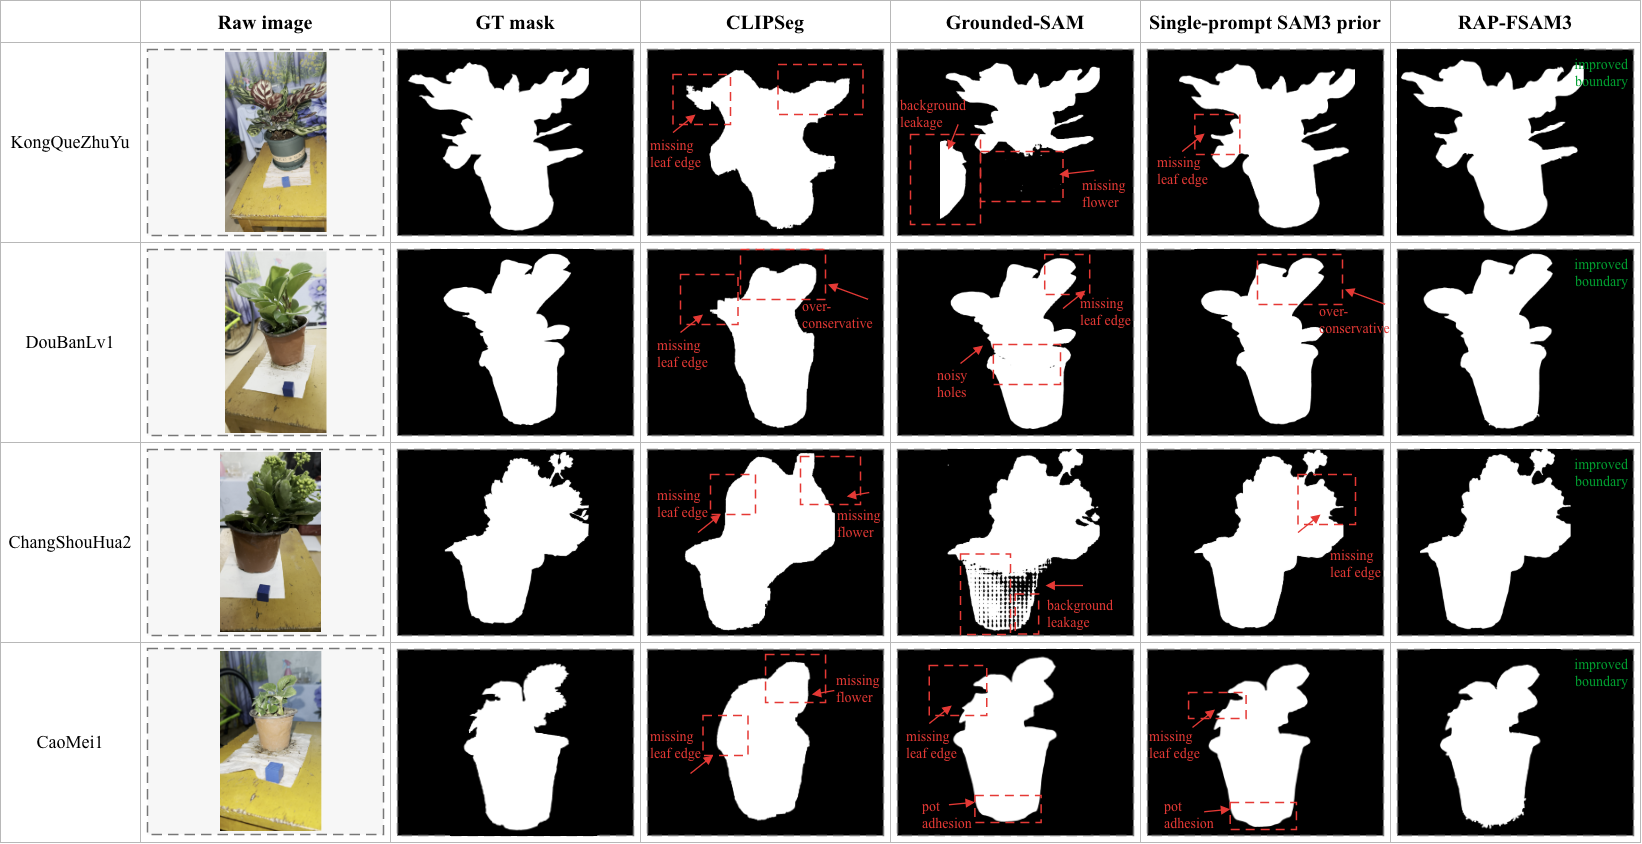
\includegraphics[width=\textwidth,height=0.46\textheight,keepaspectratio]{Fig3.png}
\caption{Qualitative comparison of VFM-based potted-plant foreground priors. RAP-FSAM3 reduces background leakage and improves boundary continuity compared with direct single-prompt and general VFM baselines.}\label{fig:vfm-comparison}
\end{figure}
\FloatBarrier

\subsection{Prompt Sensitivity Reveals Semantic Bias in Direct VFM Prompting}\label{sec:prompt-robustness-results}

We then evaluated the stability of direct VFM prompting. The plant-instance prompt was the most stable direct prompt, with F1 = 0.9692 on the same manually annotated evaluation frames. Its masks often retained the visible pot together with the plant, indicating that the VFM interpreted the target as a complete potted-plant foreground instance rather than a plant-body-only object. The green-region prompt reached F1 = 0.7972 but was prone to including green background regions. In contrast, the organ-level prompt showed under-recall, the seedling-oriented prompt failed systematically on mature or mixed-structure plants, and the background-excluding plant prompt was overly conservative. These results show that single-prompt VFM segmentation is semantically fragile in potted-plant scenes. The prompt robustness results are summarised in Table~\ref{tab:prompt-robustness}, and representative prompt failure modes are shown in Fig.~\ref{fig:prompt-failure}.

\begin{table}[pos=!htbp]
\caption{Prompt robustness of direct VFM foreground extraction on the same manually annotated evaluation frames.}\label{tab:prompt-robustness}
\centering
\scriptsize
\setlength{\tabcolsep}{4pt}
\resizebox{\textwidth}{!}{%
\begin{tabular}{@{}llll@{}}
\toprule
Prompt type & Text prompt & F1 $\uparrow$ & Main behaviour \\
\midrule
Green-region prompt & \texttt{green plant} & 0.7972 & Prone to green-background inclusion \\
Plant-instance prompt & \texttt{entire potted plant} & 0.9692 & Most stable foreground-instance prompt; includes visible pot support \\
Organ-level prompt & \texttt{leaves and stems} & 0.6471 & Under-recall for mixed or thick structures \\
Seedling-oriented prompt & \texttt{crop seedling} & 0.0768 & Near-empty masks on mature plants \\
Background-excluding plant prompt & \texttt{plant body without background} & 0.4051 & Over-conservative foreground extraction \\
\bottomrule
\end{tabular}%
}
\end{table}

\begin{figure}[pos=!htbp]
\centering
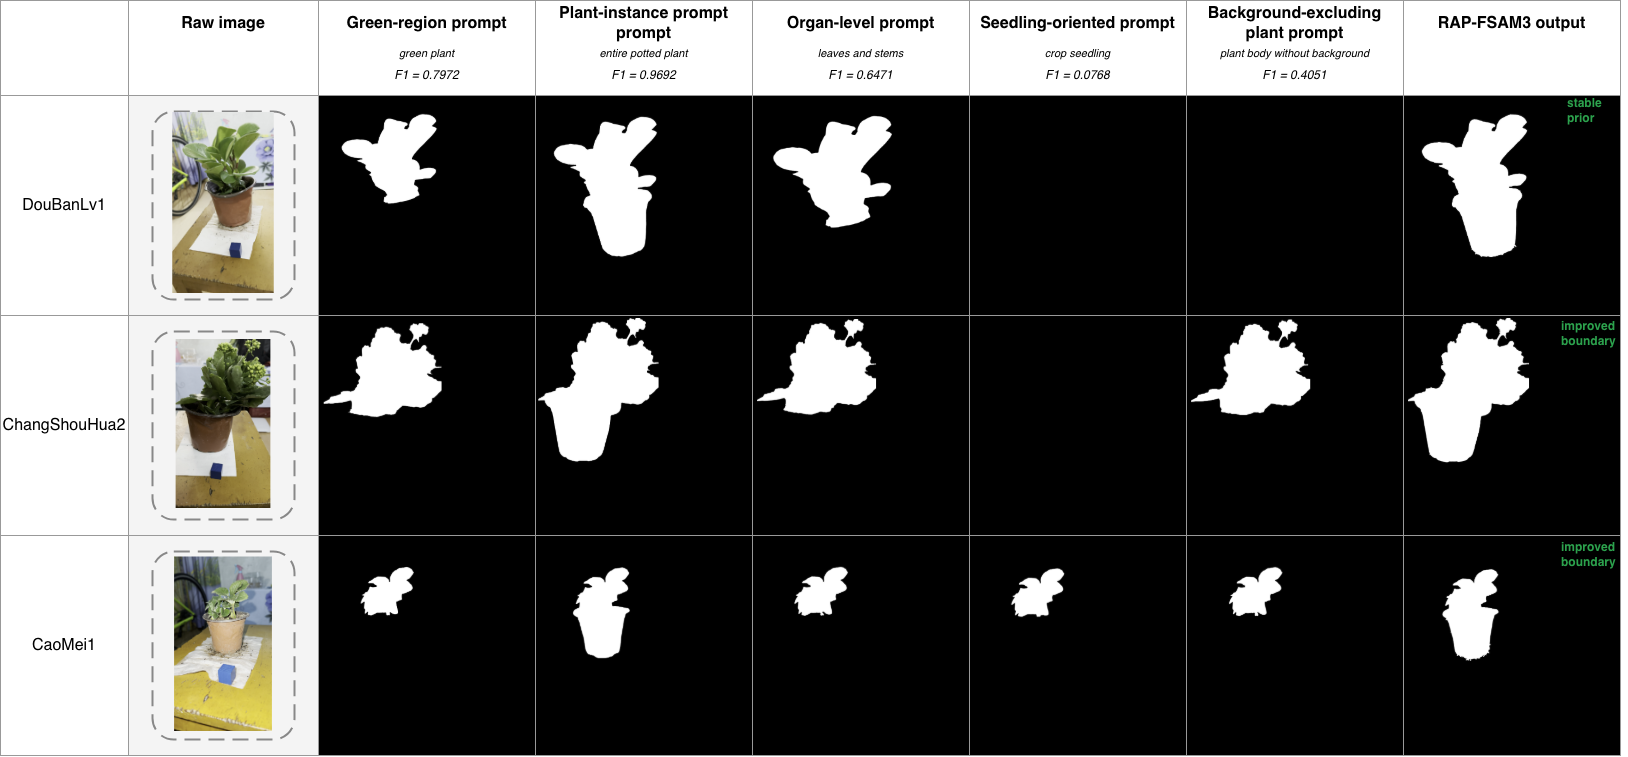
\includegraphics[width=\textwidth,height=0.46\textheight,keepaspectratio]{Fig4.png}
\caption{Prompt sensitivity of direct VFM segmentation in potted-plant scenes. Single-prompt outputs exhibit semantic bias across plant forms, motivating prompt-adaptive foreground-prior generation.}\label{fig:prompt-failure}
\end{figure}
\FloatBarrier

\subsection{Ablation of RAP-FSAM3 Adaptation Modules}\label{sec:rap-ablation-results}

We further evaluated the RAP-FSAM3 adaptation components on the same manually annotated evaluation frames. The fixed plant-instance prompt served as the direct single-prompt baseline and corresponds to the Single-prompt SAM3 prior in Table~\ref{tab:vfm-comparison}. To test whether multi-prompt selection was reliable by itself, we included a diagnostic geometry-only multi-prompt selector without semantic gating. This variant selected semantically inappropriate candidates in several frames and degraded F1, mIoU, HD95 and Boundary-F1, even though leakage energy alone did not fully reflect the missing-foreground failure. After semantic gating was introduced, the selected prior recovered the stable plant-instance prompt under this evaluation protocol, producing the same evaluated masks as the fixed prompt while avoiding the geometry-only failure mode. Structure-balanced foreground--background refinement improved boundary quality and leakage suppression, and the complete RAP-FSAM3 with geometry-consistency foreground correction achieved the best overall metrics, matching the final RAP-FSAM3 result reported in Table~\ref{tab:vfm-comparison}. The module ablation is shown in Table~\ref{tab:rap-ablation}.

\begin{table}[pos=!htbp]
\caption{Ablation of RAP-FSAM3 adaptation components on the same manually annotated evaluation frames. The geometry-only selector is a diagnostic variant used to evaluate the necessity of semantic-gated multi-prompt selection. The fixed plant-instance prompt and the full RAP-FSAM3 correspond to the shared baseline and final method in Table~\ref{tab:vfm-comparison}.}\label{tab:rap-ablation}
\centering
\scriptsize
\setlength{\tabcolsep}{3pt}
\resizebox{\textwidth}{!}{%
\begin{tabular}{@{}lcccccccc@{}}
\toprule
Setting & SG-MPS & SB-FBPR & GCFC & F1 $\uparrow$ & mIoU $\uparrow$ & HD95 / px $\downarrow$ & Boundary-F1 $\uparrow$ & Leakage energy $\downarrow$ \\
\midrule
Fixed plant-instance prompt & -- & -- & -- & 0.9692 & 0.9624 & 193.71 & 0.4051 & 0.002272 \\
Geometry-only multi-prompt selector w/o SG-MPS & No & -- & -- & 0.8429 & 0.8533 & 1008.90 & 0.3214 & 0.002035 \\
Semantic-gated selected prior & Yes & -- & -- & 0.9692 & 0.9624 & 193.71 & 0.4051 & 0.002272 \\
RAP-FSAM3 w/o GCFC & Yes & Yes & No & 0.9677 & 0.9613 & 190.70 & 0.4543 & 0.001935 \\
RAP-FSAM3 (ours, full) & Yes & Yes & Yes & \textbf{0.9706} & \textbf{0.9641} & \textbf{183.42} & \textbf{0.4643} & \textbf{0.001739} \\
\bottomrule
\end{tabular}%
}
\begin{flushleft}
\scriptsize SG-MPS: semantic-gated multi-prompt selection; SB-FBPR: structure-balanced foreground--background prompt refinement; GCFC: geometry-consistency foreground correction.
\end{flushleft}
\end{table}

\FloatBarrier


\subsection{VFM-Prior Injection into 2DGS Is Necessary for Foreground-Object Reconstruction}\label{sec:injection-ablation-results}

The ForeSplat objective-level injection mechanism is summarised in Fig.~\ref{fig:algorithm}, and the micro-level M2M3-GO controller is illustrated in Fig.~\ref{fig:m2m3-go-micro}. To determine whether VFM-derived plant priors must be used during training, we compared full-scene 2DGS, input-domain foreground masking, opacity-only regularisation, foreground-object loss injection, complete ForeSplat with and without M2M3-GO, and post hoc mask pruning on a representative broad-leaf foreground morphology. The unconstrained full-scene baseline reconstructed nearly the entire background, with an outside-mask non-black ratio of 0.9908 and a leakage energy ratio of 1.2201. Input-domain foreground masking reduced background visibility but decreased PSNR\_fg from 24.2090 dB to 20.7291 dB, indicating substantial foreground-quality loss. Alpha mask consistency, background opacity suppression and their joint regularisation did not prevent background learning when full-image RGB supervision was retained. Foreground-object loss injection reduced the outside ratio and leakage below the foreground-only thresholds. Adding M2M3-GO to the complete ForeSplat objective produced a modest refinement in foreground PSNR\_fg, leakage suppression and Gaussian count, indicating primitive-level capacity adjustment rather than a decisive foreground-separation effect. In contrast, post hoc mask pruning after full-scene training reduced the number of primitives but still left a high outside ratio and leakage energy, showing that training-after-processing pruning cannot replace training-time foreground-object optimisation. The core metrics are listed in Table~\ref{tab:injection-ablation}, and the visual evidence is shown in Fig.~\ref{fig:injection-ablation}.

\begin{figure}[pos=!htbp]
\centering
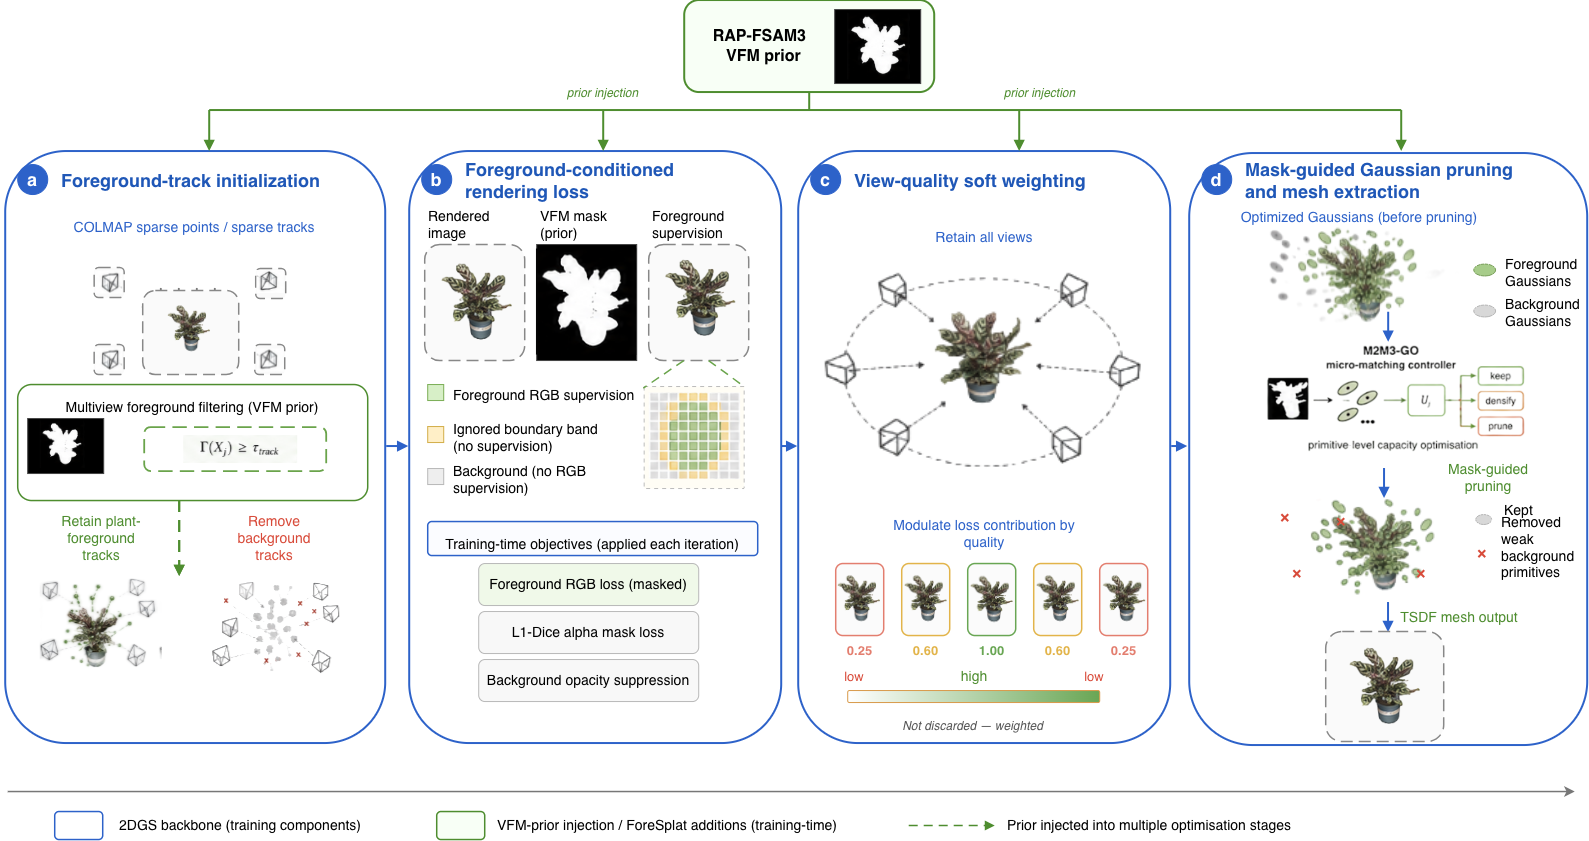
\includegraphics[width=\textwidth,height=0.46\textheight,keepaspectratio]{Fig5.png}
\caption{Foreground-object optimisation with a lightweight M2M3-GO refinement layer. RAP-FSAM3 foreground priors are injected into sparse-track initialisation, foreground-conditioned rendering losses, opacity constraints and view-quality weighting. After the foreground-object target has been established, M2M3-GO converts pixel-level masks into primitive-level Gaussian utility scores through mask-to-model support, model-to-mask coverage deficit and boundary support, supporting keep, densify and prune decisions before mesh extraction. The module is used as a refinement layer rather than as an independent compression component.}\label{fig:algorithm}
\end{figure}

\FloatBarrier

\begin{table}[pos=!htbp,abovecap=2pt,belowcap=2pt,abovetbl=2pt,belowtbl=0pt]
\caption{Ablation of VFM-prior injection positions in 2DGS optimisation on a representative broad-leaf foreground morphology.}\label{tab:injection-ablation}
\centering
\scriptsize
\setlength{\tabcolsep}{3pt}
\resizebox{\textwidth}{!}{%
\begin{tabular}{@{}lccccccccc@{}}
\toprule
Method setting & FG init. & FG RGB & Alpha/bg & M2M3-GO & PSNR\_fg $\uparrow$ & Outside ratio $\downarrow$ & Leakage $\downarrow$ & Gaussian count $\downarrow$ & Foreground only \\
\midrule
Full-scene 2DGS & No & No & No & No & 24.2090 & 0.9908 & 1.2201 & 751,213 & No \\
Input-domain foreground masking & No & Implicit & No & No & 20.7291 & 0.0073 & 0.0042 & 263,108 & Yes, with quality loss \\
Alpha mask consistency only & No & No & Alpha & No & 24.3422 & 0.9898 & 1.2260 & 768,067 & No \\
Background opacity suppression only & No & No & Background & No & 24.7508 & 0.9900 & 1.2255 & 742,931 & No \\
Joint alpha and background opacity regularisation & No & No & Joint & No & 24.8126 & 0.9896 & 1.2266 & 763,266 & No \\
Foreground-object loss injection & No & Yes & Joint & No & 25.0072 & 0.0294 & 0.0190 & 592,900 & Yes \\
Complete ForeSplat objective w/o M2M3-GO & Yes & Yes & Joint & No & 25.0478 & 0.0298 & 0.0193 & 596,840 & Yes \\
Complete ForeSplat objective & Yes & Yes & Joint & Yes & \textbf{25.1055} & \textbf{0.0294} & \textbf{0.0189} & 591,623 & Yes \\
Post hoc mask pruning after full-scene training & No & No & Post hoc & No & 24.6918 & 0.7509 & 0.7900 & 468,920 & No \\
\bottomrule
\end{tabular}%
}

\begin{flushleft}
\scriptsize Complete ForeSplat objective w/o M2M3-GO keeps all foreground-object training components except the primitive-level M2M3-GO controller. Post hoc mask pruning is placed as a training-after-processing reference, because it removes primitives only after full-scene Gaussian capacity has already formed.
\end{flushleft}
\end{table}

\FloatBarrier

The comparison between the complete ForeSplat objective and its w/o M2M3-GO variant further evaluates the role of primitive-level refinement. Removing M2M3-GO led to a small decrease in PSNR\_fg and leakage suppression, while the reconstruction still remained foreground-only. This indicates that the dominant foreground-object separation is achieved by foreground RGB supervision and opacity constraints, whereas M2M3-GO provides a modest refinement to Gaussian-level capacity allocation after the foreground-object reconstruction target has been defined. Therefore, M2M3-GO is treated as an optimisation-time primitive controller rather than an independent compression or reconstruction module. Fig.~\ref{fig:m2m3-go-micro} illustrates the corresponding micro-level controller.

\begin{figure}[pos=!htbp]
\centering
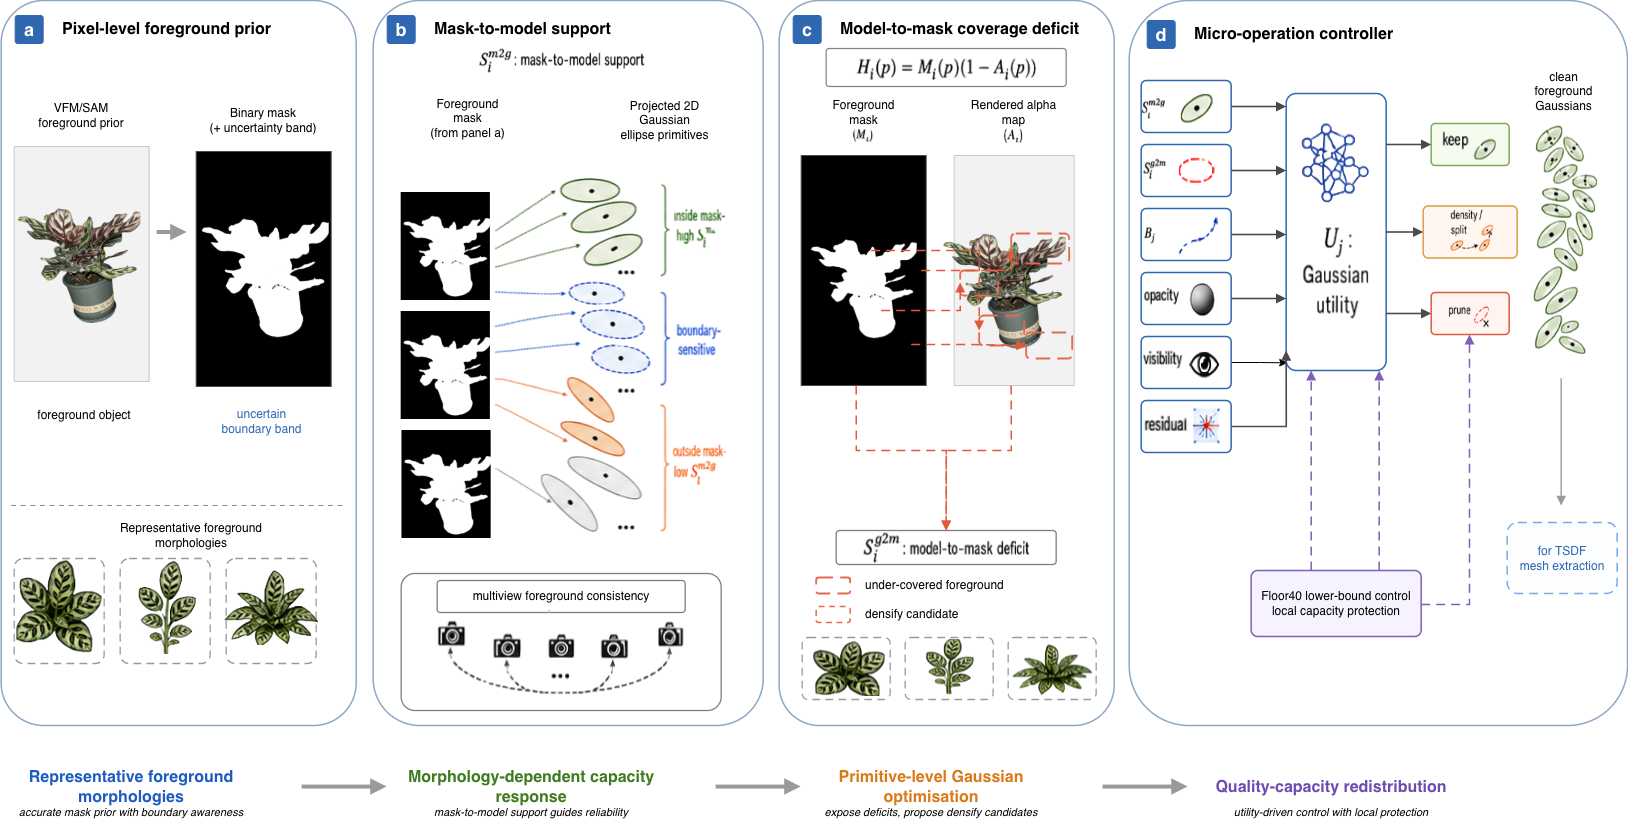
\includegraphics[width=\textwidth,height=0.46\textheight,keepaspectratio]{Fig6.png}
\caption{Micro-level M2M3-GO primitive refinement mechanism. The module bridges pixel-level foreground priors and Gaussian-level operations by computing mask-to-model support, model-to-mask coverage deficit and boundary support for each primitive. These cues are integrated into a Gaussian utility score that controls keep, densify and prune decisions. Broad-leaf, compact flowering and low-canopy foreground patterns are shown as mechanism examples, while the Floor40 gate denotes an optional local lower-bound safeguard against over-aggressive primitive removal.}\label{fig:m2m3-go-micro}
\end{figure}

\FloatBarrier

The qualitative comparison in Fig.~\ref{fig:injection-ablation} complements the quantitative ablation by showing how training-time prior injection differs from input masking and post hoc pruning in the rendered foreground region.

\begin{figure}[pos=!htbp]
\centering
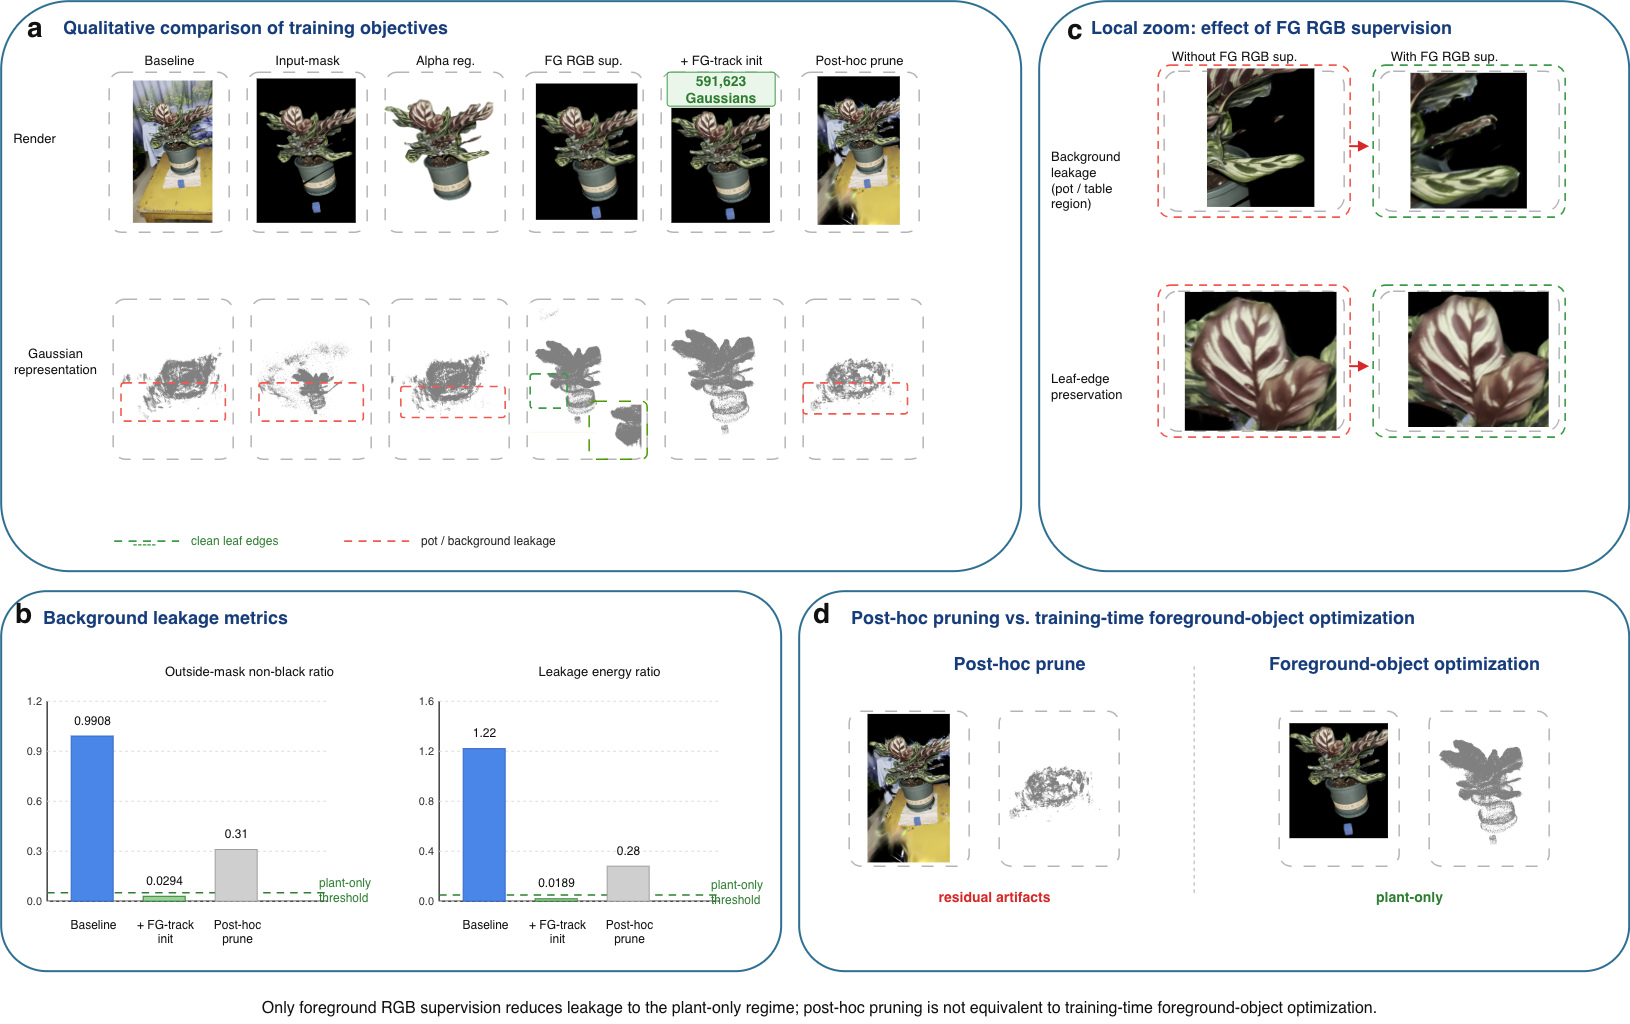
\includegraphics[width=\textwidth,height=0.46\textheight,keepaspectratio]{Fig7.png}
\caption{Visual evidence for VFM-prior injection in 2DGS. Training-time foreground-object optimisation suppresses background learning more effectively than input masking or post hoc pruning.}\label{fig:injection-ablation}
\end{figure}

\FloatBarrier



\subsection{Workflow-Level Reconstruction, Mesh Generation and Phenotypic Validation}\label{sec:workflow-validation-results}

ForeSplat stably generated measurable 3D representations from ordinary RGB acquisition. All samples completed the full workflow from video capture, RAP-FSAM3 masking, COLMAP, 2DGS and TSDF meshing to phenotypic measurement. The workflow-level comparison in Table~\ref{tab:reconstruction} should be interpreted as an application-level baseline comparison under a unified input and runtime protocol, rather than as a pure loss-function ablation. COLMAP, 3DGS with VFM foreground preprocessing and standard 2DGS serve as reconstruction baselines, whereas ForeSplat explicitly reformulates the task as foreground-object reconstruction for plant phenotyping. Under the same 20-sequence evaluation protocol, ForeSplat achieved PSNR = 31.09 dB, SSIM = 0.9711 and LPIPS = 0.0365. Compared with standard 2DGS, the complete workflow increased PSNR by 1.51 dB and reduced training/reconstruction time and mesh-extraction time by 60.94\% and 65.17\%, respectively. Compared with 3DGS with VFM foreground preprocessing, ForeSplat maintained higher reconstruction quality while reducing mesh-extraction time from 642 s to 55 s. Representative reconstruction and mesh examples are shown in Fig.~\ref{fig:reconstruction}.

\begin{table}[pos=!htbp]
\caption{Workflow-level reconstruction quality and processing efficiency under a unified 20-sequence protocol. Values are averaged over all 20 RGB sequences. The same input frame sampling, train/test view split, image resolution and computing environment were used for all methods whenever applicable. Neural-rendering methods were trained for 30,000 iterations.}\label{tab:reconstruction}
\centering
\scriptsize
\setlength{\tabcolsep}{3pt}
\resizebox{\textwidth}{!}{%
\begin{tabular}{@{}lccccc@{}}
\toprule
Method & PSNR $\uparrow$ & SSIM $\uparrow$ & LPIPS $\downarrow$ & Train/recon time / s $\downarrow$ & Meshing time / s $\downarrow$ \\
\midrule
COLMAP & 13.63 & 0.8745 & 0.1072 & 599.5 & 78 \\
3DGS with VFM foreground preprocessing & 30.17 & 0.9587 & 0.0386 & 5413.5 & 642 \\
Standard 2DGS & 29.58 & 0.9574 & 0.0487 & 12913.7 & 157.9 \\
ForeSplat & \textbf{31.09} & \textbf{0.9711} & \textbf{0.0365} & 5044.5 & \textbf{55.0} \\
\bottomrule
\end{tabular}%
}
\begin{flushleft}
\scriptsize Runtime columns report stage-level wall-clock time measured on the same workstation with two NVIDIA RTX A6000 GPUs (48 GB each) and 128 GB system memory. Train/recon time denotes neural optimisation time for 3DGS/2DGS-based methods and sparse-reconstruction runtime for COLMAP; meshing time denotes only mesh extraction. VFM foreground-prior generation, frame extraction, manual measurement and I/O are not included in these two timing columns.
\end{flushleft}
\end{table}

\begin{figure}[pos=!htbp]
\centering
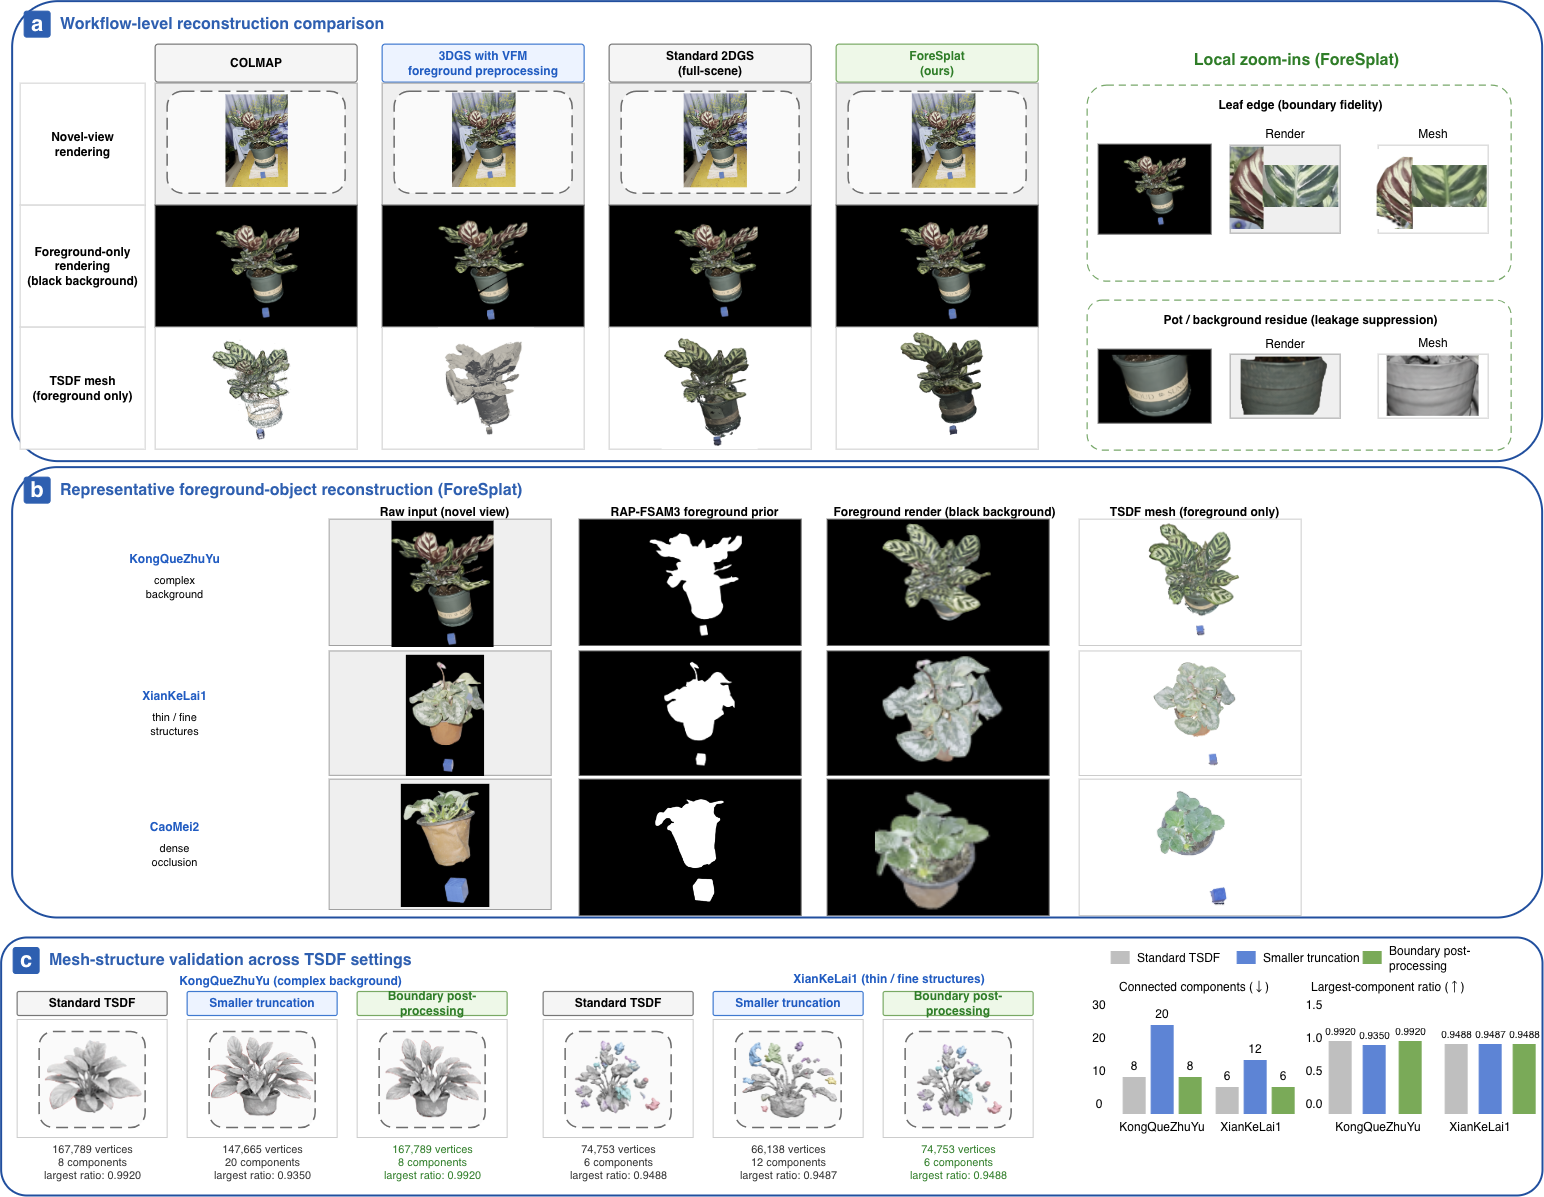
\includegraphics[width=\textwidth,height=0.46\textheight,keepaspectratio]{Fig8.png}
\caption{Representative reconstruction and mesh outputs. ForeSplat reduces background residue and produces foreground-object meshes suitable for virtual phenotypic measurement.}\label{fig:reconstruction}
\end{figure}

\FloatBarrier

The reconstructed 3D representations were further used for agricultural trait measurement. Virtual measurements were compared with manual measurements for plant height, canopy width, leaf length and leaf width. ForeSplat achieved strong agreement for plant-level structural traits, with \(R^2\) values of 0.988 for plant height and 0.988 for canopy width. The mean MAPE of the two plant-level traits was 5.71\%. Leaf-level traits showed slightly larger relative errors, with a mean MAPE of 8.59\% across leaf length and leaf width. Leaf width had the lowest \(R^2\) value of 0.900, but its absolute error remained moderate, with an MAE of 0.45 cm and an RMSE of 0.64 cm. This pattern indicates that leaf width is more sensitive to local boundary uncertainty and its narrower value range, rather than representing a complete failure of the virtual measurement pipeline. The quantitative results are listed in Table~\ref{tab:phenotyping}, and the scatter plots and residual distributions are shown in Fig.~\ref{fig:phenotyping}.

\begin{table}[pos=!htbp]
\caption{Agreement between manual and virtual phenotypic measurements across all plant samples. Plant height and canopy width were evaluated at the plant level (n = 21), while leaf length and leaf width were evaluated on three representative leaves per plant (n = 63). Bias is defined as virtual measurement minus manual measurement. \(R^2\) values are rounded to three decimal places.}\label{tab:phenotyping}
\centering
\scriptsize
\setlength{\tabcolsep}{3pt}
\resizebox{\textwidth}{!}{%
\begin{tabular}{@{}lcccccc@{}}
\toprule
Trait & n & MAE/cm $\downarrow$ & RMSE/cm $\downarrow$ & MAPE/\% $\downarrow$ & Bias/cm & \(R^2\) $\uparrow$ \\
\midrule
Plant height & 21 & 0.98 & 1.21 & 6.91 & 0.58 & 0.988 \\
Canopy width & 21 & 0.86 & 0.99 & 4.50 & 0.64 & 0.988 \\
Leaf length & 63 & 0.51 & 0.64 & 7.45 & 0.31 & 0.974 \\
Leaf width & 63 & 0.45 & 0.64 & 9.73 & 0.38 & 0.900 \\
\bottomrule
\end{tabular}%
}
\end{table}

\begin{figure}[pos=!htbp]
\centering
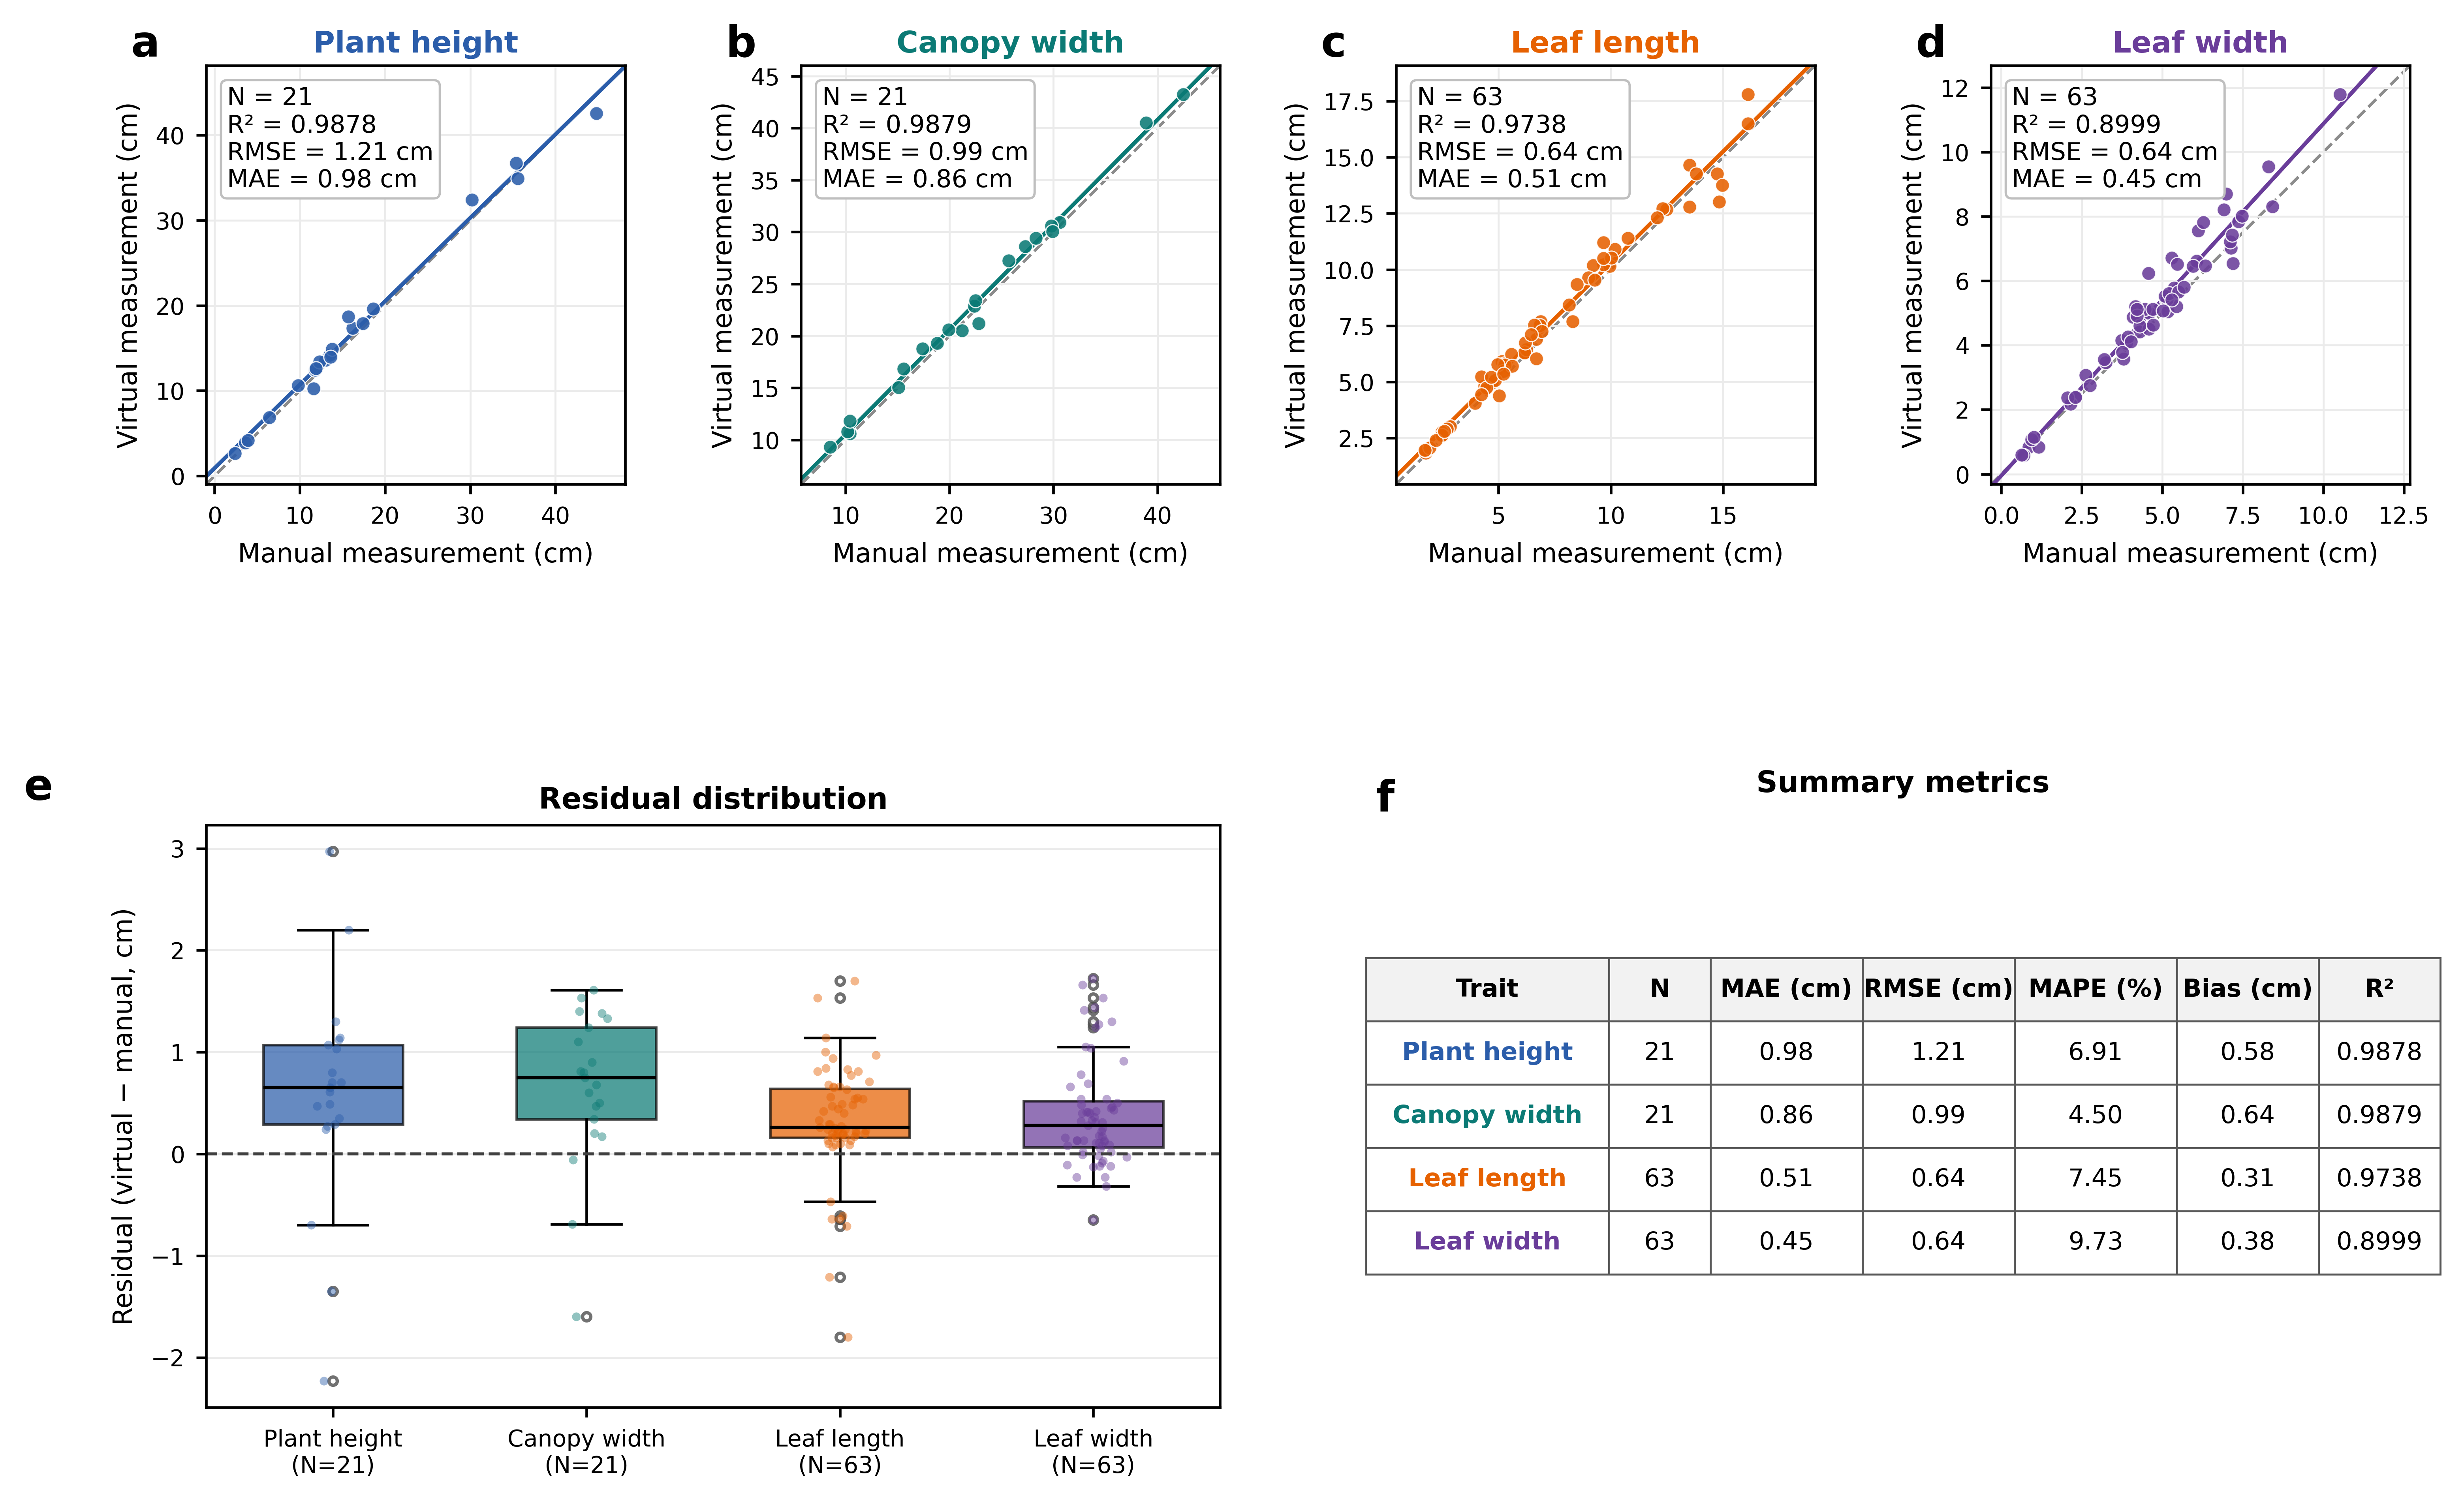
\includegraphics[width=\textwidth,height=0.46\textheight,keepaspectratio]{Fig9.png}
\caption{Agreement between manual measurements and virtual phenotypic measurements. Scatter plots, residual distributions and summary metrics show that ForeSplat supports plant height, canopy width, leaf length and leaf width measurement.}\label{fig:phenotyping}
\end{figure}

\FloatBarrier

\section{Discussion}\label{sec:discussion}

\subsection{Vision Foundation Models Require Agricultural Prompt Adaptation}\label{sec:vfm-prompt-adaptation}

The VFM experiments show that direct prompting is not a stable interface for potted-plant foreground generation, consistent with recent evidence that SAM-style foundation models require task-aware prompting, post-processing or adaptation when transferred to agricultural and other real-world segmentation settings \cite{ref65,ref66,ref67}. The plant-instance prompt was effective on average because it matched the way the VFM grouped the plant and visible pot as one foreground instance, but organ-level, seedling-oriented and overly conservative background-excluding prompts exposed clear semantic bias. RAP-FSAM3 addresses this problem by treating VFM outputs as candidate foreground priors rather than final masks. Semantic-gated multi-prompt selection prevents semantically inconsistent prompt choices; structure-balanced foreground--background refinement explicitly suppresses table, neighbouring-object and background interference while retaining the visible support base when it is consistently part of the foreground instance; and geometry-consistency correction adds conservative geometric support near difficult boundaries. Thus, RAP-FSAM3 is best understood as an agricultural task adapter for frozen VFMs rather than as a new foundation model.

\subsection{Foreground Priors Should Define the 3D Optimisation Target}\label{sec:vfm-priors-to-3d-objective}

The central finding of the 2DGS ablation is that foreground-object representations for trait measurement cannot be reliably obtained by mask pruning after full-scene training. During standard 2DGS optimisation, background regions generate photometric gradients and form stable Gaussian capacity through densification. Post hoc pruning can remove only some primitives after they have formed; it cannot redirect capacity allocation during training. The failure of opacity-only constraints shows that constraining the opacity field alone is insufficient when full-image RGB supervision is retained. Only when RGB supervision itself is restricted to foreground pixels does the main optimisation pressure shift towards the plant object. This supports the view that VFM-derived masks should be converted into 3D reconstruction objectives rather than used only as image preprocessing or post-processing cues, which is consistent with recent efforts to make object segmentation part of Gaussian optimisation rather than only a post hoc query step \cite{ref70}.


\subsection{From Foreground-Object Supervision to Primitive-Level Capacity Allocation}\label{sec:primitive-level-capacity-allocation}

The M2M3-GO analysis clarifies that foreground-object reconstruction involves two coupled optimisation levels. The first level is image-domain objective reformulation, where foreground RGB supervision and opacity constraints redirect the main photometric gradients towards the target potted-plant instance. The second level is primitive-domain capacity refinement, where Gaussian primitives are densified, preserved or removed according to their multiview foreground support and contribution to under-covered foreground regions. M2M3-GO addresses the second level by converting mask-to-model support, model-to-mask coverage deficit and boundary proximity into primitive-level micro-decisions.

M2M3-GO is therefore best understood as a lightweight primitive-level refinement component within ForeSplat. It complements foreground RGB supervision and opacity constraints by refining how Gaussian primitives are allocated once the mask-defined reconstruction target has been established. The ablation in Table~\ref{tab:injection-ablation} shows a modest improvement rather than a dominant foreground-separation effect, which is consistent with its role as a refinement layer. Compactness is not treated as a standalone guarantee; instead, the controller prioritises measurement-relevant foreground support and uses the Floor40 gate only as a local safeguard against over-pruning boundary-sensitive or locally sparse structures.


\subsection{Phenotyping-Oriented Reconstruction and Boundary-Sensitive Traits}\label{sec:phenotyping-boundary-errors}

Plant height and canopy width are determined by overall bounding ranges and are therefore less sensitive to local boundary errors. Leaf length depends on the main axis of individual leaves and has intermediate difficulty. Leaf width depends on local cross-sectional boundaries and is most affected by reconstruction resolution, Gaussian support domains, TSDF fusion and landmark placement. This error pattern is consistent with recent 3D plant phenotyping studies in which global architectural traits are usually more stable than local organ-level traits under boundary uncertainty \cite{ref57,ref58}. The lower \(R^2\) for leaf width indicates that local boundary quality remains the main limiting factor for fine-grained virtual phenotyping, especially because leaf width has a narrower dynamic range than plant height or canopy width.

The remaining measurement errors mainly arise from three sources. First, boundary-sensitive traits such as leaf width depend on the local completeness of thin leaf margins, where small segmentation deviations or TSDF fusion artefacts can translate into centimetre-level landmark shifts. Second, scale recovery relies on the physical reference in the reconstructed scene, so small endpoint-selection or mesh-boundary deviations can propagate to all virtual measurements. Third, manual measurements are used as the operational reference, but repeated operator measurements were not separately collected in this study. Therefore, the current validation demonstrates agreement with standard manual measurements, but it does not fully decompose reconstruction error, scale-recovery uncertainty and manual-measurement variability. Future work should include repeated manual measurements, scale-marker repeatability analysis and Bland--Altman agreement analysis on independent greenhouse or field datasets. These additions would further clarify whether the virtual-measurement error remains below the practical uncertainty of routine manual phenotyping.

\subsection{Relationship to Reference Studies}\label{sec:relationship-to-reference-studies}

Compared with IPENS \cite{ref35} and LCR-GS \cite{ref34}, ForeSplat does not extract target point clouds or individual-plant subsets after reconstruction. Instead, it converts VFM-derived potted-plant foreground priors into training-time constraints and directly produces a foreground-object Gaussian representation. Compared with general Gaussian Grouping \cite{ref36} and SAGA-style semantic lifting \cite{ref37}, ForeSplat focuses on an agricultural measurement objective: whether the reconstructed foreground object is suitable for plant-trait extraction. These routes are not mutually exclusive. Future systems could combine stronger feature matching, SAM2/3 temporal propagation, LCR-GS-style multi-plant decomposition and ForeSplat foreground-object optimisation for more complex greenhouse and field scenes.

\section{Conclusion}\label{sec:conclusion}

We present ForeSplat, a VFM-guided foreground-object 2D Gaussian Splatting workflow for low-cost 3D plant phenotyping. RAP-FSAM3 adapts vision foundation models to potted-plant foreground-prior generation through semantic-gated multi-prompt selection, structure-balanced foreground--background prompt refinement and geometry-consistency foreground correction. ForeSplat further injects these priors into the 2DGS training objective through foreground-track initialisation, foreground RGB supervision, alpha and background opacity constraints, view-quality-aware soft loss weighting, a lightweight M2M3-GO primitive-level refinement layer and mask-guided Gaussian pruning. The results show that direct single-prompt VFM segmentation is sensitive to prompt semantics, while RAP-FSAM3 improves boundary consistency and leakage suppression. Foreground-object loss injection is the key mechanism for suppressing background learning in 2DGS, and input masking or post hoc pruning alone is insufficient. Validation across 20 sequences and 21 plants indicates that the workflow can support low-cost measurement of plant height, canopy width, leaf length and leaf width under indoor or semi-controlled potted-plant conditions. Overall, ForeSplat demonstrates that vision foundation models can support agricultural 3D phenotyping when their outputs are adapted as reconstruction-aware foreground priors and converted into 3D optimisation constraints. M2M3-GO further provides a lightweight primitive-level refinement step for Gaussian keep, densify and prune decisions within the foreground-object reconstruction process.

\section*{Funding}
\addcontentsline{toc}{section}{Funding}

This research was supported by the Special Fund of Chinese Central Government for Basic Scientific Research Operations in Commonweal Research Institutes (Nos. JBYW-AII-2026-46, JBYW-AII-2026-47, JBYW-AII-2026-06, JBYW-AII-2026-58, JBYW-AII-2026-13 and Y2026JC11).

\section*{Data Availability}
\addcontentsline{toc}{section}{Data Availability}

The multiview RGB sequences, manually annotated foreground-prior evaluation frames, RAP-FSAM3 masks, phenotypic measurement tables, view-weight files and main running configurations supporting this study will be released through a project repository or data repository after data curation is complete. The released configuration files will include the foreground-prior prompt settings, foreground-prior selection thresholds, loss weights, M2M3-GO parameters, view-quality weighting settings and mask-guided pruning parameters. Before public release, the data and configuration files are available from the corresponding author upon reasonable request.
https://github.com/LiuLiShenShe/ForeSplat.git

\section*{Ethics Statement}
\addcontentsline{toc}{section}{Ethics Statement}

This study involved only plant imaging and measurement. It did not involve human or animal subjects.

\section*{Competing Interests}
\addcontentsline{toc}{section}{Competing Interests}

The authors declare no competing interests.

\bibliographystyle{elsarticle-num-names}
\bibliography{cas-refs}

\end{document}
